\documentclass[11pt]{exam}
\usepackage{amsmath}
\usepackage{amssymb}
\usepackage{graphicx}
\usepackage{gensymb}
\usepackage{enumitem}
\usepackage{amsfonts}
\usepackage{amssymb}
\usepackage{ifthen}
\usepackage{geometry}
\usepackage{siunitx}
\usepackage{mdframed}
\usepackage{amsthm}
\usepackage{titlesec}
\setcounter{secnumdepth}{4}
\titleformat{\paragraph}
{\normalfont\normalsize\bfseries}{\theparagraph}{1em}{}
\titlespacing*{\paragraph}
{0pt}{3.25ex plus 1ex minus .2ex}{1.5ex plus .2ex}

\usepackage{xparse}
\usepackage{hyperref}
\usepackage{color}
\usepackage{tcolorbox}
\noprintanswers

\usepackage{tikz}
\usetikzlibrary{shapes,backgrounds}
\usepackage[all]{xy}
\usepackage{pgfplots}
%\pgfplotsset{compat=1.6}
\pgfplotsset{soldot/.style={color=blue,only marks,mark=*}} \pgfplotsset{holdot/.style={color=blue,fill=white,only marks,mark=*}}

\addtolength{\textheight}{3cm}
\addtolength{\topmargin}{-1cm}
\addtolength{\textwidth}{3cm}
\addtolength{\oddsidemargin}{-1.5cm}
\addtolength{\evensidemargin}{-1.5cm}
\setlength\parindent{0pt}

\newcommand {\DS} [1] {${\displaystyle #1}$}
\newcommand{\ds}{\displaystyle}
\newcommand{\vv}{\vspace{.2cm}}
\newcommand{\answer}[1]{\textcolor{blue}{#1}}
\newcommand{\R}{\mathbb{R}}
\newcommand{\C}{\mathbb{C}}
\newcommand{\Z}{\mathbb{Z}}
\newcommand{\N}{\mathbb{N}}
\newcommand{\link}[2]{\href{#1}{\textcolor{blue}{#2}}}
\pagestyle{empty}
\usepackage{mathtools}
\DeclarePairedDelimiter{\norm}{\lVert}{\rVert}
\newcommand{\vectorproj}[2][]{\textit{proj}_{\vect{#1}}\vect{#2}}
\newcommand{\vect}{\mathbf}

%============================================

%============================================

\definecolor{137cp1}{RGB}{13, 33, 161}
\definecolor{137cp2}{RGB}{51, 161, 253}
\definecolor{137cp3}{RGB}{255, 67, 101}
\definecolor{137cp4}{RGB}{232, 144, 5}


%============================================

%============================================

\usepackage{hyperref}
\hypersetup{colorlinks}
\hypersetup{urlcolor=137cp3, linkcolor=137cp1}


%============================================

%============================================

\newcommand{\M}[2]{\Omega^{\, #2}_{\, #1}}

\DeclareMathOperator{\Walt}{Walt}
\DeclareMathOperator{\Tor}{Tor}


%%%%%%%%%%%%%%%%%%%%%%%%%%%%%%%%%%%%%%%%%

\begin{document}
\begin{center}
{\huge PHY252 Course Notes}
\end{center}
\section{Energy in Thermal Physics}
\subsection{Thermal Equilibrium}
\hspace*{10mm}After two objects have been in contact long enough, we say that they are in thermal equilibrium. The time required for a system to come to thermal equilibrium is called the relaxation time. In a second type of equilibrium, diffusive equilibrium, the molecules of each substance are free to move around but no longer have any tendency to move one way or another. In mechanical equilibrium, large scale motions can take place but no longer do. For each type of equilibrium between two systems, there is a quantity that can be exchanged between the systems 
\begin{table}[htp]
\centering
\begin{tabular}{cc} 
Exchanged quantity & Type of equilibrium \\ 
\hline
energy & thermal \\
volume & mechanical \\
particles & diffusive
\end{tabular}
\label{default}
\end{table}\\
\hspace*{10mm}When two objects are able to exchange energy, and energy tends to move spontaneously from one to the other, we say that the object that gives up energy is at a higher temperature, and the object that absorbs energy is a lower temperature. As such, we define temperature as the measure of the tendency of an object to spontaneously give up energy to its surroundings. When two objects are in thermal contact, the one that tends to spontaneously lose energy is at the higher temperature. \\
\hspace*{10mm}For any low-density gas at constant pressure, the volume should go to zero at approximately $-273\degree\text{C}$. Alternatively, if the volume of the gas is fixed, then its pressure will approach zero as the temperature approaches $-273\degree\text{C}$. This special temperature is called absolute zero, and defines the zero-point of the absolute temperature scale. The SI unit of absolute temperature is called the kelvin. A kelvin is the same size as a degree Celsius, but kelvin temperatures are measured up from absolute zero instead of from the freezing point of water. 
\newpage
\subsection{The Ideal Gas}
Many of the properties of a low-density gas can be summarized in the ideal gas law, 
\begin{equation}\tag{1.1}
PV=nRT
\end{equation}
where $P=$ pressure, $V=$ volume, $n=$ number of moles of gas, $R$ is a universal constant, and $T$ is the temperature in kelvins. The constant $R$ in the ideal gas law has the empirical value 
\begin{equation}\tag{1.2}
R=8.31\frac{\text{J}}{\text{mol}\cdot\text{K}}
\end{equation}
in SI units, that is, measuring pressure in N/m$^2$ = Pa\;(pascals) and volume in m$^3$. A mole of molecules is Avogadro's number of them, 
\begin{equation}\tag{1.3}
N_A = 6.02\times 10^{23}.
\end{equation}
As such, we denote the number of molecules by capital $N$:
\begin{equation}\tag{1.4}
N=n\times N_A.   
\end{equation}
Substituting $N/N_A$ for $n$ in the ideal gas law and combining $R/N_A$ as a new constant, we obtain 
\begin{equation}\tag{1.5}
PV=NkT
\end{equation}
The constant $k$ called Boltzmann's constant is small when expressed in SI units since Avogadro's number is large:
\begin{equation}\tag{1.6}
k=\frac{R}{N_A}=1.381\times 10^{-23} J/K.
\end{equation}
\hspace*{10mm}For a given amount of has at a given temperature, doubling the pressure squeezes the gas into exactly half as much space. Similarly, at a given volume, doubling the temperature causes the pressure to double.\\
\hspace*{10mm}The ideal gas law is an approximation, never exactly true for a real gas in the real world. It is valid in the limit of low density, when the average space between gas molecules is much larger than the size of a molecule. 
\newpage
\subsubsection*{Microscopic Model of an Ideal Gas}
\hspace*{10mm}Let us first construct a cylinder containing just one gas molecule, as shown in Figure 1. The length of the cylinder is $L$, the area of the piston is $A$, and therefore the volume inside is $V=LA$. At the moment, the molecule has a velocity vector $\vec{v}$ with horizontal component $v_x$. As time passes, the molecule bounces off the walls of the cylinder, so its velocity changes. However, assume that these collisions are always elastic, so the molecule doesn't lose any kinetic energy; its speed never changes. Further assume that the surfaces of the cylinder and piston are perfectly smooth, so the molecule's path as it bounces is symmetrical about a line normal to the surface. \\
\hspace*{10mm}To determine how the temperature of a gas is related to the kinetic energy of the molecules it contains, we must first figure out how pressure is related to kinetic energy; then invoke the ideal gas law to relate pressure to temperature.  
\begin{figure}[htp]
    \centering
    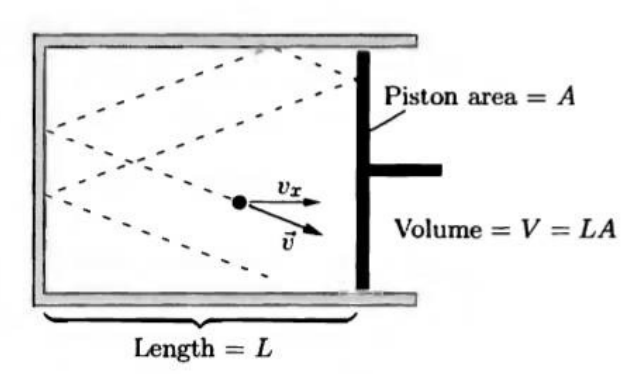
\includegraphics[width=5cm]{figure1.png}
    \caption{A simplified model of an ideal gas, with just one molecule bouncing around elastically.}
\label{fig:simplified_piston}
\end{figure}\\
\hspace*{10mm}Pressure means force per unit area, exerted in this case on the piston and the other walls of the cylinder. Usually the pressure exerted on the piston by the molecule is zero since the molecule isn't even touching the piston, but periodically the molecule crashes into the piston and bounces off exerting a relatively large force on the piston for a brief moment. As such, we calculate the average pressure as follows:
\begin{equation}\tag{1.9}
\overline{P} = \frac{\overline{F_x}_{\text{,on piston}}}{A}=\frac{-\overline{F_x}_{\text{,on molecule}}}{A}=-\frac{m\left(\frac{\overline{\Delta v_x}}{\Delta t}\right)}{A}
\end{equation}
The pressure was first written in terms of the $x$ component of the force exerted by the molecule on the piston. Then, Newton's third law was used to write the pressure in terms of the force exerted by the piston on the molecule. Finally, Newton's second law was used to replace the force by the mass $m$ of the molecule times its acceleration, $\Delta v_x/ \Delta t$. To include only those accelerations caused by the piston, we take $\Delta t$ to be exactly the time it takes for the molecule to undergo one round-trip from the left to the right and back again:
\begin{equation}\tag{1.10}
\Delta t = 2L/v_x.
\end{equation}
(Collisions with the perpendicular walls will not affect the molecule's motion in the $x$ direction.) During this time interval, the molecule undergoes exactly one collision with the piston, and the change in its $x$ velocity is 
\begin{equation}\tag{1.11}
\Delta v_x = (v_{x,\text{ final}}) - (v_{x,\text{ initial}}) = (-v_x)-(v_x)=-2v_x.
\end{equation}
Putting these expressions into equation 1.9, we find for the average pressure on the piston
\begin{equation}\tag{1.12}
\overline{P} = -\frac{m}{A}\frac{(-2v_x)}{(2L/v_x)}=\frac{mv_x^2}{AL}=\frac{mv_x^2}{V}.
\end{equation}
\hspace*{10mm}Now, suppose that the cylinder contains some large number, $N$, of identical molecules, with random positions and directions. We further assume that the molecules don't collide or interact with each other - just with the walls. Since each molecule periodically collides with the piston, the average pressure is given by a sum of terms of the form of the form of equation 1.12. 
\begin{equation}\tag{1.13}
\overline{P}V=mv_{1x}^2 + mv_{2x}^2 + mv_{3x}^2 + \cdots    
\end{equation}
If the number of molecules is large, the collisions will be so frequent that that the pressure is essentially continuous. On the other hand, the sum of $v_x^2$ for all $N$ molecules is $N$ times the average of their $v_x^2$ values. So using the average over all molecules, equation 1.13 then becomes 
\begin{equation}\tag{1.14}
PV = Nm\overline{v_x^2}. 
\end{equation}
Then invoking the ideal gas law (1.8) as an experimental fact allows us to substitute $NkT$ for $PV$ on the left-hand side of equation 1.14. So we obtain 
\begin{equation}\tag{1.15}
kT = m\overline{v_x^2}\quad\text{or}\quad\overline{\frac{1}{2}mv_x^2} = \frac{1}{2}kT
\end{equation}
where the left-hand side is almost equal to the average translational kinetic energy of the molecules with the only problem being the $x$ subscript which can be removed by realizing the equation also holds for $y$ and $z$:
\begin{equation}\tag{1.16}
\overline{\frac{1}{2}mv_y^2} = \overline{\frac{1}{2}mv_z^2} = \frac{1}{2}kT
\end{equation}
The average translational kinetic energy is then 
\begin{equation}\tag{1.17}
\overline{K}_\text{trans}=\overline{\frac{1}{2}mv^2}= \frac{1}{2}m(\overline{v_x^2+v_y^2+v_z^2})=\frac{1}{2}kT + \frac{1}{2}kT +\frac{1}{2}kT = \frac{3}{2}kT.
\end{equation}
(Note that the average of a sum is the sum of the averages.)\\
\hspace*{10mm}The average translational kinetic energy of the molecules in a gas is given by a simple constant times the temperature. If this model is accurate, the temperature of a gas is a direct measure of the average translational kinetic energy of its molecules.\\
\hspace*{10mm}Since Boltzmann's constant $k$ has unit, J/K, to convert s temperature into an energy, $k$ is a conversion factor between temperature and molecular energy, at least for this simple system. Since the joule is not a convenient unit for dealing with small energies, we often use the electron-volt (eV), which is the kinetic energy of an electron that has been accelerated through a voltage difference of one volt: 1 eV = $1.6\times 10^{-19}$ J. Boltzmann's constant is $8.62\times 10^{-5}$ eV/K, so at room temperature, 
\begin{equation}\tag{1.19}
kT =  (8.62\times 10^{-5} \text{ eV/K})(300\;\text{K}) = 0.026 \text{ eV}\approx \frac{1}{40} \text{ eV}.
\end{equation}\\
\hspace*{10mm}The average speed of the molecules in a gas can almost be obtained from equation 1.17, but not quite. Solving for $\overline{v^2}$ gives 
\begin{equation}\tag{1.20}
\overline{v^2}=\frac{3kT}{m},   
\end{equation}
but if we take the square root of both sides, we get not the average speed, but rather the square root of the average of the speeds:
\begin{equation}\tag{1.21}
v_{\text{rms}} \equiv \sqrt{\overline{v^2}} = \sqrt{\frac{3kT}{m}}.   
\end{equation}
We further see that $v_{\text{rms}}$ is only slightly larger than $\overline{v}$ so $v_{\text{rms}}$ is a fine estimate of the average speed. According to equation 1.21, light molecules tend to move faster than heavy ones, at a given temperature.
\newpage
\hspace*{10mm}Note the result, equation 1.17, breaks down if molecules exert forces on each other, or if collisions with the walls are inelastic, or if the ideal gas law itself fails. Brief interactions between molecules are generally no issue, since such collisions won't change the average velocities of the molecules. The only serious problem is when the gas becomes so dense that the space occupied by the molecules themselves becomes a substantial fraction of the total volume of the container. In this case, however, the ideal gas law also breaks down, in such a way as to preserve equation 1.17. Consequently, this equation is still true, not only for dense gases but also most liquids and some solids.
\newpage
\subsection{Equipartition of Energy}
\hspace*{10mm}The equipartition theorem concerns all forms of energy for which the formula is a quadratic function of a coordinate or velocity component. Each such form of energy is called a degree of freedom. In addition to translational motion in the $x$, $y$, $z$ directions, other degrees of freedom might include rotational motion, vibrational motion, and elastic potential energy (as stored in a spring). The equipartition theorem states that at temperature $T$, the average energy of any quadratic degree of freedom is $\frac{1}{2}kT$. If a system contains $N$ molecules, each with $f$ degrees of freedom, and there are no other (non-quadratic) temperature-dependent forms of energy, then its total thermal energy is 
\begin{equation}\tag{1.23}
U_{\text{thermal}}= N\cdot f \cdot \frac{1}{2}kT.
\end{equation}
Technically this is just the average total thermal energy, but if $N$ is large, fluctuations away from the average will be negligible.\\
\hspace*{10mm}The quantity $U_{\text{thermal}}$ is almost never the total energy of a system; there's also static energy that doesn't change as we change the temperature, such as energy stored in chemical bonds or the rest energies ($mc^2$) of all the particles in the system. So it's safest to apply the equipartition theorem only to changes in energy when the temperature is raised or lowered, and to avoid phase transformations and other reactions in which bonds between particles may be broken. \\
\hspace*{10mm}In a gas of monatomic molecules like helium or argon, only translational motion counts, so each molecule has three degrees of freedom, that is, $f=3$. In a diatomic gas like oxygen (O$_2$) or nitrogen (N$_2$), each molecule can also rotate about two different axes, see Figure 2. Rotation about the axis running down the length of the molecule doesn't count, for reasons having to do with quantum mechanics. The same is true for carbon dioxide (CO$_2$), since it also has an axis of symmetry down its length.
\begin{figure}[htp]
    \centering
    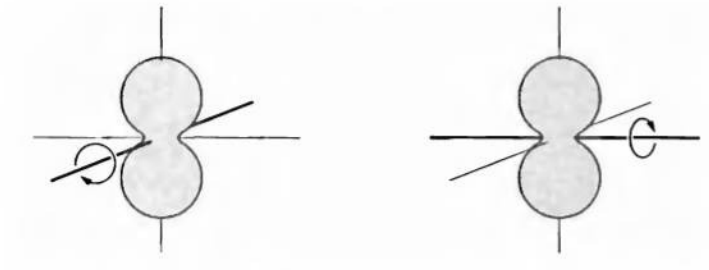
\includegraphics[width=5cm]{figure2.png}
    \caption{A diatomic molecule can rotate about two independent axes, perpendicular to each other. Rotation about the third axis, down the length of the molecule, is not allowed.}
\label{fig:diatomic_molecule}
\end{figure}\\
\hspace*{10mm}To observe why a rotational degree of freedom has the same average energy as a translational degree of freedom, suppose gas molecules inside a container are knocking around and colliding with each other and with the walls. We see that the average rotational energy should eventually reach some equilibrium value that is larger if the molecules are moving fast (high temperature) and smaller if the molecules are moving slow (low temperature). In any particular collision, rotational energy might be converted to translational energy or vice versa, but on average these processes should balance out. \\
\hspace*{10mm}A diatomic molecule can also vibrate, as if the two atoms were held together by a spring. This vibration should count as two degrees of freedom, one for the vibrational kinetic energy and one for the potential energy. (Recall from classical mechanics that the average kinetic energy and potential energies of a simple harmonic oscillator are equal - a result that is consistent with the equipartition theorem. More complicated molecules can vibrate in a variety of ways: stretching, flexing, twisting. Each mode of vibration counts as two degrees of freedom. \\
\hspace*{10mm}However, at room temperature many vibrational degrees of freedom do not contribute to a molecule's thermal energy. For instance, air molecules (N$_2$ and O$_2$), have only five degrees of freedom, not seven, at room temperature. At higher temperatures, the vibrational modes do eventually contribute. We say that these modes are frozen out at room temperature; evidently, collisions with other molecules are sufficiently violent to make an air molecule rotate, but not hardly ever violent enough to make it vibrate. \\
\hspace*{10mm}In a solid, each atom can vibrate in three perpendicular directions, so for each atom there are six degrees of freedom (three for kinetic energy and three for potential energy). A simple model of a crystalline solid is shown in Figure 3. If we let $N$ stand for the number of atoms and $f$ stand for the number of degrees of freedom per atom, then we can use equation 1.23 with $f=6$ for a solid. However, some of the degrees may be frozen out at room temperature. 
\begin{figure}[htp]
    \centering
    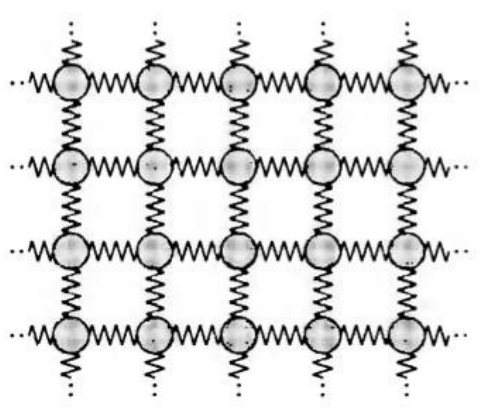
\includegraphics[width=5cm]{figure3.png}
    \caption{The bed-spring model of a crystalline solid. Each atom is like a ball, joined to its neighbours by springs. In three dimensions, there are six degrees of freedom per atom}
\label{fig:crystalline_solid}
\end{figure}\\
\hspace*{10mm}Liquids are more complicated then either gases or solids. We can generally use the formula $\frac{3}{2}kT$ to find the average translational kinetic energy of molecules in a liquid, but the equipartition theorem doesn't work for the rest of the thermal energy, because the intermolecular potential energies are not quadratic functions. \\
\hspace*{10mm}To test the equipartition theorem, we would have to add some energy to a system, measure how much its temperature changes, and compare to equation 1.23. 
\newpage
\subsection{Heat and Work}
\hspace*{10mm}Fundamentally, temperature is a measure of an object's tendency to spontaneously give up energy. Since energy is the most fundamental dynamical concept in physics, we many only list the various forms of energy - kinetic, electrostatic, gravitational, chemical, nuclear - and state the law of conservation of energy. The law of conservation of energy says that, while energy can often be converted from one form to another, the total amount of energy in the universe never changes. Although there are many mechanisms by which energy can be put into or taken out of a system, in thermodynamics, we classify these mechanisms under two categories: heat and work. \\
\hspace*{10mm}Heat is defined as any spontaneous flow of energy from one object to another, caused by a difference in temperature between the objects. The mechanism may be different in each case, but in each process the energy transferred is called heat. \\
\hspace*{10mm}Work, in thermodynamics, is defined as any other transfer of energy into or out of a system. With work, we can identify some agent (possibly an inanimate object) that is actively putting energy into the system; it wouldn't happen automatically. \\
\hspace*{10mm}Both heat and work refer to energy in transit. In addition to the total energy inside a system, we can only discuss how much heat entered a system, or how much work done on a system. \\
\hspace*{10mm}We will use the symbol $U$ for the total energy inside a system, and $Q$ and $W$ will represent the amount of energy that enters a system as heat and work, respectively, during any time period of interest. (Either one could be negative, if energy leaves the system.) Then, the sum $Q+W$ is the total energy that enters the system, and, by conservation of energy, is the amount by which the systems energy changes (see Figure 4). Written as an equation, 
\begin{equation}\tag{1.24}
\Delta U = Q + W,    
\end{equation}
the change in energy equals the heat added plus the work done. This equation is known as the first law of thermodynamics. 
\begin{figure}[htp]
    \centering
    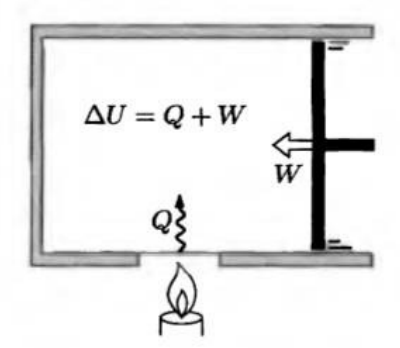
\includegraphics[width=5cm]{figure4.png}
    \caption{The total change in the energy of a system is the sum of the heat added to it and the work done on it.}
\label{fig:first_law}
\end{figure}\\
\hspace*{10mm}The official SI unit of energy is the joule, defined as 1 kg$\cdot$m$^2$/s$^2$. However, heat has traditionally been measured in calories, where 1 cal was defined as the amount of heat needed to raise the temperature of a gram of water by 1$\degree$C (while no work is being done on it). The calorie is now defied to equal exactly 4.186 J. \\
\hspace*{10mm}Processes of heat transfer are further classified into three categories, according to the mechanism involved. Conduction is the transfer of heat by molecular contact: Fast-moving molecules bump into slow-moving molecules, giving up some of their energy in the process. Convection is the bulk motion of a gas or liquid, usually driven by the tendency of warmer material to expand and rise in a gravitational field. Radiation is the emission of electromagnetic waves, mostly infrared for objects at room temperature but including visible light for hotter objects like the filament of a lightbulb or the surface of the sun. 
\newpage
\subsection{Compression Work}
The most important type of work is work done on a system (often a gas) by compressing it, as when a piston is pushed. In such a case, the amount of work done is equal to the force you exert dotted into the displacement:
\begin{equation}\tag{1.25}
W = \vec{F}\cdot \vec{d}r.
\end{equation}
(In thermodynamics, $\vec{d}r$ always refers to the point of contact). In this case the work-energy theorem says that the total energy of the system increases by $W$. \\
\hspace*{10mm}Since it's more convenient to express the work done in terms of the pressure and volume for a gas, for definiteness, consider the typical cylinder-piston arrangement shown in Figure 5. The force is parallel, so
\begin{equation}\tag{1.26}
W=F\Delta x.    
\end{equation}
where $\Delta x$ is positive when the piston moves inward. 
\begin{figure}[htp]
    \centering
    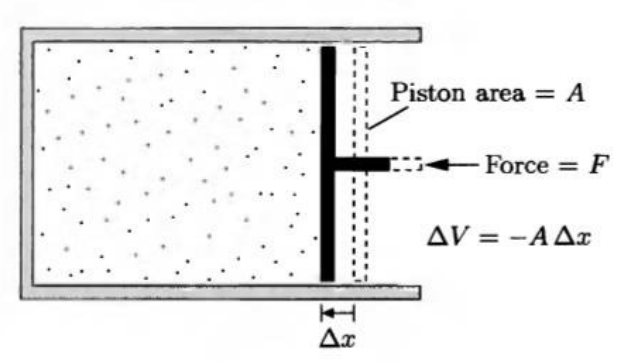
\includegraphics[width=5cm]{figure5.png}
    \caption{When the piston moves inward, the volume of the gas changes by $\Delta V$ (a negative amount) and the work done on the gas (assuming quasistatic compression) is $-P\Delta V$.}
\label{fig:quasistatic}
\end{figure}\\
\hspace*{10mm}To replace $F$ by $PA$, the pressure of the gas times the area of the piston, assume that as the gas is compressed it always remains in internal equilibrium, so that its pressure is uniform from place to place (and hence well defined). For this to be true, the piston's motion must be reasonably slow, so that the gas has time to continually equilibrium to the changing conditions. A volume change that is slow in this sense is termed quasistatic. Although perfectly quasistatic compression is an idealization, it is usually a good approximation in practice. To compress the gas non-quasistatically, we must slam the piston very hard, so it moves faster than the gas can respond (the speed must be at least comparable to the speed of sound in the gas). \\
\hspace*{10mm}For quasistatic compression, then, the force exerted on the gas equals the pressure of the gas times the area of the piston. Thus 
\begin{equation}\tag{1.27}
W=PA\Delta x \quad \text{(for quasistatic compression).}    
\end{equation}
But the product $A\Delta x$ is minus the change in the volume of the gas (minus because the volume decreases when the piston moves in), so 
\begin{equation}\tag{1.28}
W=-P\Delta V \quad\text{(quasistatic).}    
\end{equation}
\newpage
\hspace*{10mm}If the pressure is constant, then the work done is minus the area under a graph of pressure vs. volume (see Figure 6). If the pressure is not constant, the process is divided into many tiny steps, the area under the graph for each step is computed, then the areas are added to get the total work. That is, the work is still minus the total area under the graph of $P$ vs. $V$.
\begin{figure}[htp]
    \centering
    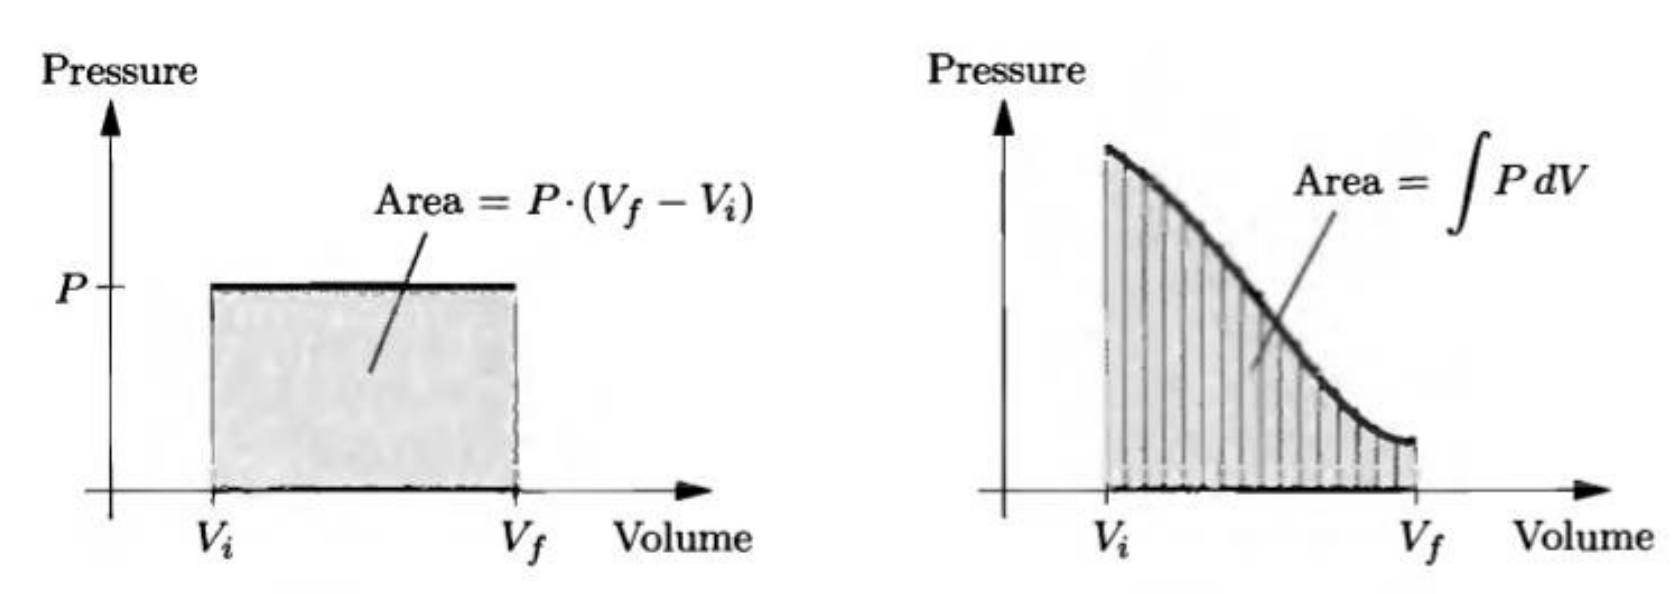
\includegraphics[width=6cm]{figure6.png}
    \caption{When the piston moves inward, the volume of the gas changes by $\Delta V$ (a negative amount) and the work done on the gas (assuming quasistatic compression) is $-P\Delta V$.}
\label{fig:quasistatic_integral}
\end{figure}\\
\hspace*{10mm}If we know the formula for the pressure as a function of volume, $P(V)$, then we can compute the total work as an integral:
\begin{equation}\tag{1.29}
W=-\int_{V_i}^{V_f} P(V)dV\quad\text{(quasistatic).}  
\end{equation}
\hspace*{10mm}Compression-expansion work is not the only type of work that can be done on thermodynamic systems. 
\newpage
\subsubsection*{Compression of an Ideal Gas}
When a container full of gas is compressed, work is done on it, that is, energy is added. Generally this causes the temperature of the gas to increase. However, if the gas is compressed very slowly, or if the container is in good thermal contact with its environment, heat will escape as the gas is compressed and its temperature won't rise very much. The difference between fast and slow compression is therefore very important in thermodynamics. \\
\hspace*{10mm}We will consider two idealized ways of compressing an ideal gas: isothermal compression, which is so slow that the temperature of the gas doesn't rise at all; and adiabatic compression, which is so fast that no heat escapes from the gas during the process. Most real compression processes will be somewhere between these two extremes, usually closer to the adiabatic approximation. \\
\hspace*{10mm}Suppose, that we compress an ideal gas isothermally, that is, without changing its temperature. This implies that the process is quasistatic, so we can use formula 1.29 to calculate the work done, with $P$ determined by the ideal gas law. On a $PV$ diagram, the formula $P=NkT/V$, for constant T, is a concave-up hyperbola (called an isotherm), as shown in Figure 7. The work done is minus the area under the graph. 
\begin{align*}\tag{1.30}
W &= -\int_{V_i}^{V_f}PdV=-NkT\int_{V_i}^{V_f}\frac{1}{V}dV\\
&=-NkT(\ln{V_f}-\ln{V_i})=NkT\ln{\frac{V_i}{V_f}}
\end{align*}    
Notice that the work done is positive if $V_i > V_f$, that is, if the gas is being compressed. If the gas expands isothermally, the same equation applies but with $V_i < V_f$, that is, the work done on the gas is negative.\\
\hspace*{10mm}As the gas is compressed isothermally, heat must be flowing out, into the environment. To calculate how much, we can use the first law of thermodynamics and the fact that for an ideal gas $U$ is proportional to $T$:
\begin{equation}\tag{1.31}
Q=\Delta U-W=\Delta(\frac{1}{2}NfkT)-W=0-W=NkT\ln{\frac{V_f}{V_i}}.
\end{equation}
\begin{figure}[htp]
    \centering
    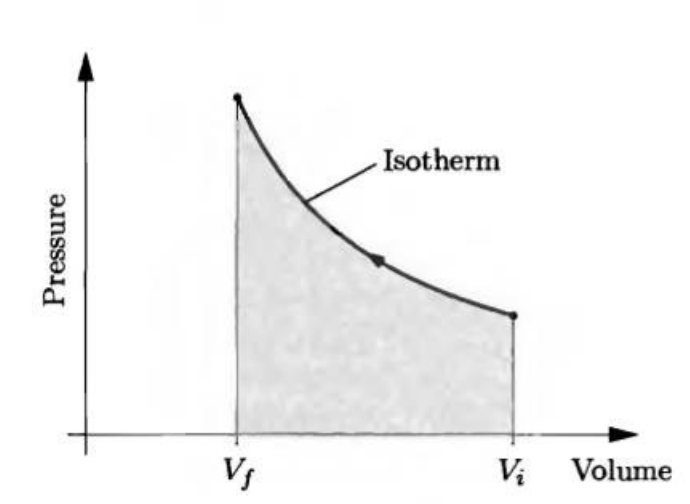
\includegraphics[width=6cm]{figure7.png}
    \caption{For isothermal compression of an ideal gas, the $PV$ graph is a concave-up hyperbola, called an isotherm. As always, the work done is minus the area under the graph.}
\label{fig:isotherm}
\end{figure}\\
Thus the heat input is just minus the work done. For compression, $Q$ is negative because heat leaves the gas; for isothermal expansion, heat must enter the gas so $Q$ is positive.\\
\hspace*{10mm}Adiabatic compression is so fast that no heat flows out of (or into) the gas. Assume, however, that the compression is quasistatic. 
\newpage
\hspace*{10mm}If work is done on a gas and heat is not allowed to escape, the internal energy of the gas will increase:
\begin{equation}\tag{1.32}
\Delta U = Q+W=W.    
\end{equation}
If it's an ideal gas, $U$ is proportional to $T$ so the temperature increases as well. The curve describing this process on a $PV$ diagram must connect a low-temperature isotherm to a high-temperature isotherm, and therefore must be steeper than either of the isotherms (see Figure 8). \\
\hspace*{10mm}To find an equation describing the exact shape of this curve, let us first use the equipartition theorem to write
\begin{equation}\tag{1.33}
U=\frac{f}{2}NkT,    
\end{equation}
where $f$ is the number of degrees of freedom per molecule - 3 for a monatomic gas, 5 for a diatomic gas near room temperature, etc. Then the energy change along any infinitesimal segment of the curve is 
\begin{equation}\tag{1.34}
dU=\frac{f}{2}NkdT.    
\end{equation}
Meanwhile, the work done during quasistatic compression is $-PdV$, so equation 1.32, applied to an infinitesimal part of the process, becomes
\begin{equation}\tag{1.35}
\frac{f}{2}NkdT=-PdV. 
\end{equation}
This differential equation relates the changes in temperature and volume during the compression process. To solve the equation, however, we need to write the pressure $P$ in terms of the variables $T$ and $V$. The needed relation is the ideal gas law; plugging in $NkT/V$ for $P$ and cancelling the $Nk$ gives 
\begin{equation}\tag{1.36}
\frac{f}{2}\frac{dT}{T}=-\frac{dV}{V}    
\end{equation}
\begin{figure}[htp]
    \centering
    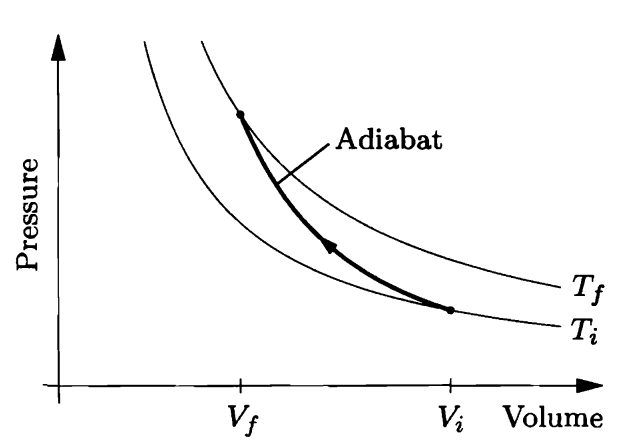
\includegraphics[width=6cm]{figure8.png}
    \caption{The $PV$ curve for adiabatic compression (called an adiabat) begins on a lower-temperature isotherm and ends on a higher-temperature isotherm.}
\label{fig:adiabat}
\end{figure}\\
\newpage
Integrating both sides from the initial values ($V_i$ and $T_i$) to the final values (($V_f$ and $T_f$)):
\begin{equation}\tag{1.37}
\frac{f}{2}\ln{\frac{T_f}{T_i}}=-\ln{\frac{V_f}{V_i}}
\end{equation}
and simplifying 
\begin{equation}\tag{1.38}
V_fT_f^{f/2}=V_iT_i^{f/2}
\end{equation}
or more compactly
\begin{equation}\tag{1.39}
VT^{f/2}=\text{constant.}
\end{equation}
To find the final pressure we can use the ideal gas law to eliminate $T$ on both sides of equation 1.38. The result can be written 
\begin{equation}\tag{1.40}
V^{\gamma}P= \text{constant,}
\end{equation}
where $\gamma$, called the adiabatic exponent, is an abbreviation for $(f+2)/f$.
\newpage
\subsection{Heat Capacities}
The heat capacity of an object is the amount of heat needed to raise its temperature, per degree temperature increase:
\begin{equation}\tag{1.41}
C\equiv \frac{Q}{\Delta T}.    
\end{equation}
(The symbol for heat capacity is a capacity is a capital $C$). The more of a substance we have, the larger its heat capacity will be. A more fundamental quantity is the specific heat capacity, defined as the heat capacity per unit mass:
\begin{equation}\tag{1.42}
    c\equiv \frac{C}{m}
\end{equation}
(The symbol for specific heat capacity is a lowercase $c$.)\\
\hspace*{10mm}The heat capacity definition (1.41) is ambiguous. The amount of heat needed to raise an object's temperature by one degree depends on the circumstances, specifically, on whether work is being done on the object (and if so, how much). Plugging the first law of thermodynamics into equation 1.41:
\begin{equation}\tag{1.43}
C=\frac{Q}{\Delta T} = \frac{\Delta U - W}{\Delta T}.     
\end{equation}
Even if the energy of an object is a well-defined function of its temperature alone (which is sometimes but not always the case), the work $W$ done on the object can be anything, so $C$ can be anything, too.\\
\hspace*{10mm}There are two types of circumstances and choices for $W$ that are most likely to occur. When $W = 0$ there is no work being done on the system. This usually means that the system's volume isn't changing, since if it were, there would be compression work equal to $-P\Delta V$. So the heat capacity, for the particular case where $W=0$ and $V$ is constant, is called the heat capacity at constant volume, denoted $C_V$. From equation 1.43, 
\begin{equation}\tag{1.44}
C_V = \left(\frac{\Delta U}{\Delta T}\right)_V = \left(\frac{\partial U}{\partial T}\right)_V.
\end{equation}
(The subscript $V$ indicates that the changes are understood to occur with the volume held fixed. The symbol $\partial$ indicates a partial derivative, in this case treating $U$ as a function of $T$ and $V$, with only $T$, not $V$ varying as the derivative is taken.) This quantity is also known as energy capacity, since it is the energy needed to raise the object's temperature per degree, regardless of whether the energy enters as heat. For a gram of water, $C_V$ is 1 cal/$\degree$C or about 4.2 J/$\degree$C.\\
\hspace*{10mm}Objects often expand as they are heated. As such, they do work on their surroundings, so $W$ is negative, so $C$ is larger than $C_V$: additional heat must be added to compensate for energy lost as work. If the pressure surrounding an object happens to be constant, then the total heat needed is unambiguous, and we refer to the heat needed per degree as $C_P$, the heat capacity at constant pressure. Plugging the formula for compression-expansion work into equation 1.43 gives
\begin{equation}\tag{1.45}
    C_P = \left(\frac{\Delta U - (-P\Delta V)}{\Delta T}\right)_P = \left(\frac{\partial U}{\partial T}\right)_P + P\left(\frac{\partial V}{\partial T}\right)_P.
\end{equation}
The last term on the right is the additional heat needed to compensate for the energy lost as work. Note that the more the volume increases, the larger this term is. For solids and liquids, $\partial V/\partial T$ is usually small and can often be neglected. For gases, however, the second term is quite significant. (The first term, $(\partial U/\partial T)_P$, is not quite the same as $C_V$, since it is $P$, not $V$, that is held fixed in the partial derivative.)\\
\hspace*{10mm}Equations 1.41 through 1.45 apply to any object whatsoever. To determine the heat capacity of some particular object, there are generally three choices: measure it; look it up in a reference work where measured values are tabulated; or try to predict it theoretically. \\
\hspace*{10mm}Suppose that a system stores thermal energy only in quadratic degrees of freedom, as described in Section 1.3. Then the equipartition theorem says $U=\frac{1}{2}NfkT$ (neglecting any "static" energy, which doesn't depend on temperature), so 
\begin{equation}\tag{1.46}
C_V = \frac{\partial U}{\partial T} = \frac{\partial}{\partial T}\left(\frac{NfkT}{2}\right) = \frac{Nfk}{2},     
\end{equation}
assuming that $f$ is independent of temperature. (Note that in this case it doesn't matter whether $V$ or $P$ is held fixed in the derivative $\partial U/\partial T$.) This result gives a direct method of measuring the number of degrees of freedom in an object, or if the number is known, of testing the equipartition theorem. For instance, in a monoatomic gas like helium, $f=3$, so we expect $C_V=\frac{3}{2}Nk = \frac{3}{2}nR$; that is, the heat capacity per mole should be $\frac{3}{2}R=12.5$ J/K. For diatomic and polyatomic molecules the heat capacity should be larger, in proportion to the number of degrees of freedom per molecule. For a solid, there are six degrees of freedom per atom, so the heat capacity per mole should be $\frac{6}{2}R=3R$; this general result is called the rule of Dulong and Petit. In this case, though, all of the degrees of freedom freeze out at low temperature, so the heat capacity approaches zero as $T\rightarrow 0$.\\
\hspace*{10mm}For an ideal gas, the derivative $\partial U/\partial T$ is the same with $P$ fixed as with $V$ fixed, and we can compute the second term in equation 1.45 using the ideal gas law. As such, the heat capacity of gasses at constant pressure is given by, 
\begin{equation}\tag{1.47}
\left(\frac{\partial V}{\partial T}\right)_P = \frac{\partial}{\partial T}\left(\frac{NkT}{P}\right)=\frac{Nk}{P}\quad\text{(ideal gas)}.    
\end{equation}
Therefore, 
\begin{equation}\tag{1.48}
C_P = C_V + Nk = C_V + nR\quad\text{(ideal gas)}.    
\end{equation}
In other words, for each mole of an ideal gas, the heat capacity at constant pressure exceeds the heat capacity at constant volume by $R$, the gas constant. The additional term in the heat capacity doesn't depend on what the pressure is, so long as it is constant. If the pressure is high the gas expands less, in such a way that the work done on the environment is independent of $P$. 
\newpage
\subsubsection*{Latent Heat}
In some situations heat can be put into a system without increasing its temperature at all. This normally happens at a phase transformation, such as melting ice or boiling water. Technically, the heat capacity is then infinite:
\begin{equation}\tag{1.49}
C=\frac{Q}{\Delta T}=\frac{Q}{0}=\infty\quad\text{(during a phase transformation).}    
\end{equation}
The amount of heat required to melt or boil a substance completely, divided by the mass of the substance, is called the latent heat of the transformation, and denoted $L$:
\begin{equation}\tag{1.50}
L\equiv \frac{Q}{m}\quad\text{to accomplish the transformation.}
\end{equation}
This definition is ambiguous, since any amount of work could also be done during the process. By convention, however, we assume that the pressure is constant (usually 1 atm), and that no other work is done besides the usual constant-pressure expansion or compression. The latent heat for melting ice is 333 J/g, or 80 cal/g. The latent heat for boiling water is 2260 J/g, or 540 cal/g. 
\newpage
\subsubsection*{Enthalpy}
Instead of discussing the energy content of a system, we can always add in the work needed to make room for it (under a constant pressure, usually 1 atm.) This work is $PV$, the pressure of the environment times the total volume of the system (that is, the total space needed to be cleared to make room for it). Adding $PV$ onto the energy gives a quantity called the enthalpy, denoted $H$:
\begin{equation}\tag{1.51}
H\equiv U + PV.    
\end{equation}
This is the total energy needed to create the system out of nothing and put it into this environment. In other words, if the system was annihilated, the energy that can be extracted is $U$ and the work ($PV$) done by the atmosphere as it collapses to fill the vacuum left behind.\\
\hspace*{10mm}Suppose that some change takes place in a system - heat is added, or chemicals react - while the pressure is always held constant. The energy, volume, and enthalpy can all change, by amounts $\Delta V$, $\Delta U$, and $\Delta H$. The new enthalpy is 
\begin{align*}\tag{1.52}
H+\Delta H &= (U + \Delta U) + P(V + \Delta V)\\
&= (U+PV) + (\Delta U + P\Delta V) \\
&= H + (\Delta U + P\Delta V),
\end{align*}
so the change in enthalpy during a constant-pressure process is 
\begin{equation}\tag{1.53}
\Delta H = \Delta U + P\Delta V\quad\text{(constant $P$).}
\end{equation}
This says that enthalpy can increase for two reasons: either because the energy increases, or because the system expands and work is done on the atmosphere to make room for it. \\
\hspace*{10mm}Recalling the first law of thermodynamics, the change in energy equals the heat added to the system, plus the compression-expansion work done on it, plus any other work (e.g., electrical) done on it:
\begin{equation}\tag{1.54}
    \Delta U = Q+(-P\Delta V) + W_{\text{other}}.
\end{equation}
Combining this law with equation 1.53, we obtain 
\begin{equation}\tag{1.55}
\Delta H = Q +  W_{\text{other}}\quad\text{(constant $P$)}, 
\end{equation}
that is, the change in enthalpy is caused only by heat and other forms of work, not by compression-expansion work (during constant-pressure processes). In other words, compression-expansion work can be ignored when dealing with enthalpy instead of energy. If no other types of work are being done, the change in enthalpy directly describes how much heat has been added to the system. (The reason why the symbol $H$ is used.)\\
\hspace*{10mm}For the case of raising an object's temperature, the change in enthalpy per degree, at constant pressure, is the same as the heat capacity at constant pressure, $C_P$: 
\begin{equation}\tag{1.56}
C_P = \left(\frac{\partial H}{\partial T}\right)_P.     
\end{equation}
This formula is the best way to define $C_P$ and is equivalent to equation 1.45. $C_P$ can be thought of as enthalpy capacity. As with $C_V$, there doesn't have to be any other heat involved at all, since the enthalpy could enter as other work, as in a microwave oven. \\
\hspace*{10mm}For each mole of water produced, $\Delta H$ for the reaction in equation 1.58 
\begin{equation}\tag{1.58}
H_2 = \frac{1}{2}O_2 \rightarrow H_2O    
\end{equation}
is -286 kJ; this quantity is referred to as the enthalpy of formation of water, because it's being formed out of elemental constituents in their most stable states. 
\newpage
\section{The Second Law}
\subsection{Two-State Systems}
Suppose three coins are flipped. There are eight possible outcomes. If the coins are fair, each outcome is equally probable, so the probability of getting three heads or three tails is one in eight. There are three different ways of getting two heads and a tail, so the probability of getting exactly two heads is 3/8, as is the probability of getting exactly one head and two tails.\\
\hspace*{10mm}Each of the eight different outcomes is called a microstate. In general, to specify the microstate of a system, we must specify the state of each individual particle, in this case the state of each coin. If we specify the state more generally, by merely saying how many heads or tails there are, we call it a macrostate. If the microstate of the system is known, the macrostate is also known. But the reverse is not true: Knowing that there are exactly two heads does not provide information about the state of each coin, since there are three microstates corresponding to the macrostate. The number of microstates corresponding to a given macrostate is called the multiplicity of that macrostate, in this case 3.\\
\hspace*{10mm}The symbol for multiplicity is the Greek letter capital omega, $\Omega$. In the preceding three coin example, $\Omega$(3 heads) = 1,  $\Omega$(2 heads) = 3, $\Omega$(1 head) = 3, and $\Omega$(0 heads) = 1. Note that the total multiplicity of all four macrostates is $1+3+3+1=8$, the total number of microstates. This quantity is referred to as $\Omega$(all). Then the probability of any particular macrostate can be written
\begin{equation}\tag{2.1}
\text{probability of $n$ heads} = \frac{\Omega(n)}{\Omega(\text{all})}.
\end{equation}
For instance, the probability of getting 2 heads is $\Omega(2)/\Omega(\text{all})=3/8$ assuming that the coins are fair and all 8 microstates are equally probable.\\
\hspace*{10mm}Now, suppose that there are 100 coins. The total number of microstates is $2^100$, since each of the 100 coins has two possible states. The number of macrostates, however, is only 101: 0 heads, 1 head, $\dots$, ... up to 100 heads. \\
\hspace*{10mm}To find the multiplicity of the $n$-heads macrostate $\Omega(n)$, we write the product of $n$ factors, starting with 100 and counting down, in the numerator. Then we divide by the product of $n$ factors, starting with $n$ and counting down to 1:
\begin{equation}\tag{2.4}
\Omega(n) = \frac{100\cdot 99\cdots(100-n+1)}{n\cdots 2\cdot1}.   
\end{equation}
The denominator is just $n$-factorial, denoted $n!$. We can also write the numerator in terms of factorials, as $100!/(100-n)!$. (This is equivalent to writing the product of all integers from 100 down to 1, then cancelling all but the first $n$ of them.) Thus the general formula can be written
\begin{equation}\tag{2.5}
\Omega(n) = \frac{100!}{n!\cdot(100-n)!}\equiv \binom{100}{n}    
\end{equation}
The last expression is the number of combinations of $n$ items chosen from 100. \\
\hspace*{10mm}If instead there are $N$ coins, the multiplicity of the macrostate with $n$ heads is
\begin{equation}\tag{2.6}
\Omega(N, n)=\frac{N!}{n!\cdot(N-n)!}=\binom{N}{n},    
\end{equation}
the number of ways of choosing $n$ objects out of $N$.
\newpage
\subsubsection*{The Two-State Paramagnet}
All materials respond in some way to a magnetic field, because of the electrical nature of electrons and atomic nuclei. A paramagnet is a material in which the constituent particles act like tiny compass needles that tend to align parallel to any externally applied magnetic field. (If the particles interact strongly enough with each other, the material can magnetize even without any externally applied field. We then call it a ferromagnet, after the most famous example, iron. Paramagnetism, in contrast, is a magnetic alignment that lasts only as long as an external field is applied.)\\
\hspace*{10mm}The individual magnetic particles are referred to as dipoles, because each has its own magnetic dipole moment vector. In practice each dipole could be an individual electron, a group of electrons in an atom, or an atomic nucleus. For any such microscopic dipole, quantum mechanics allows the component of the dipole moment vector along any given axis can take on only certain discrete values - intermediate values are not allowed. In the simplest case only two values are allowed, one positive and the other negative. We then have a two-state paramagnet, in which each elementary compass needle can have only two possible orientations, either parallel or antiparallel to the applied field. This system is drawn in Figure 9 as a bunch of little arrows each pointing either up or down. 
\begin{figure}[htp]
    \centering
    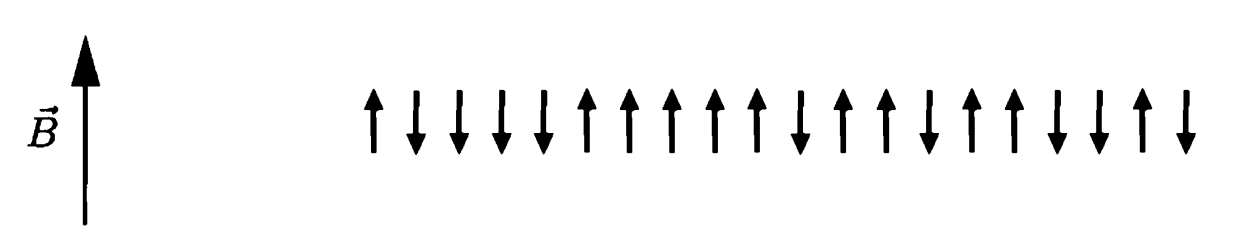
\includegraphics[width=6cm]{2statePara.png}
    \caption{A symbolic representation of a two-state paramagnet, in which each elementary dipole can point either parallel or antiparallel to the externally applied magnetic field.}
\label{fig:two-state-paramagnet}
\end{figure}\\
\hspace*{10mm}Define $N_{\uparrow}$ to be the number of elementary dipoles that point up (at some particular time), and $N_{\downarrow}$ to be the number of dipoles that point down. The total number of dipoles is then $N=N_{\uparrow} + N_{\downarrow}$, and consider this number to be fixed. This system has one macrostate for each possible value of $N_{\uparrow}$, from $0$ to $N$. The multiplicity of any macrostate is given by the formula:
\begin{equation}\tag{2.7}
\Omega(N_{\uparrow}) = \binom{N}{N_{\uparrow}} = \frac{N!}{N_{\uparrow}!N_{\downarrow}!}.    
\end{equation}
\hspace*{10mm}The external magnetic field exerts a torque on each little dipole, trying to twist it to point parallel to the field. If the external field points up, then an up-dipole has less energy than a down-dipole, since energy must be added to twist it from up to down. The total energy of the system (neglecting any interactions between dipoles) is determined by the total numbers of up- and down-dipoles, so specifying which macrostate the system is in is the same as specifying its total energy. In nearly all physical examples, the macrostate of a system is characterized, at least in part, by its total energy. 
\newpage
\subsection{The Einstein Model of a Solid}
Consider a collection of microscopic systems that can each store any number of energy units, all of the same size. Equal-size energy units occur for any quantum-mechanical harmonic oscillator, whose potential energy function has the form $\frac{1}{2}k_sx^2$ (where $k_s$ is the spring constant). The size of the energy units is then $hf$, where $h$ is Plank's constant $\num{6.63e-34}\;\text{J$\cdot$s}$ and $f$ is the natural frequency of the oscillator $(\frac{1}{2\pi}\sqrt{k_s/m})$. An abstract representation of a collection of many such oscillators in shown in Figure 10. 
\begin{figure}[htp]
    \centering
    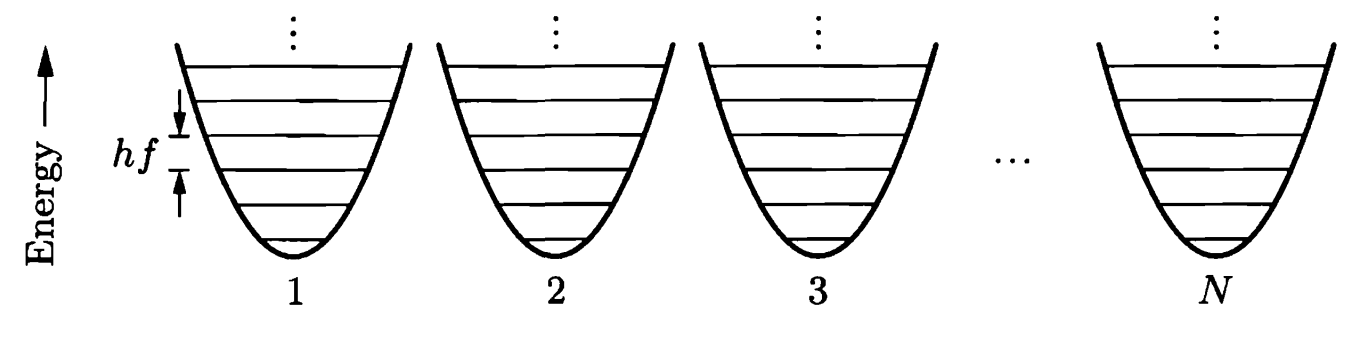
\includegraphics[width=6cm]{figure10.png}
    \caption{In quantum mechanics, any system with a quadratic potential energy function has evenly spaced energy levels separated in energy by $hf$, where $f$ is the classical oscillation frequency. An Einstein solid is a collection of $N$ such oscillators all with the same frequency.}
\label{fig:einstein-solid}
\end{figure}\\
\hspace*{10mm}In a three-dimensional solid, each atom can oscillate in three independent, so if there are $N$ oscillators, there are only $N/3$ atoms. This model of a solid as a collection of identical oscillators with quantized energy units is referred to as an Einstein solid.\\
\hspace*{10mm}The table below lists the various microstates that a system containing only three oscillators: $N=3$ could have, in order of increasing total energy; each row in the table corresponds to a different microstate. There is one microstate with total energy 0, three microstates with one unit of energy, six with two units, and ten with three units. That is 
\begin{equation}\tag{2.8}
\Omega(0) = 1,\quad\Omega(1) = 3,\quad\Omega(2) = 6,\quad\Omega(3) = 10.
\end{equation}
\begin{table}[htp]
\centering
\begin{tabular}{cccc} 
Oscillator: & $\#1$ & $\#2$ & $\#3$\\ 
\hline
Energy: & 0 & 0 & 0\\
        & 1 & 0 & 0\\
        & 0 & 1 & 0\\
        & 0 & 0 & 1\\
        & 2 & 0 & 0\\
        & 0 & 2 & 0\\
        & 0 & 0 & 2\\
        & 1 & 1 & 0\\
        & 1 & 0 & 1\\
        & 0 & 1 & 1
\end{tabular}
\quad
\begin{tabular}{cccc} 
Oscillator: & $\#1$ & $\#2$ & $\#3$\\ 
\hline 
Energy: & 3 & 0 & 0\\
        & 0 & 3 & 0\\
        & 0 & 0 & 3\\
        & 2 & 1 & 0\\
        & 2 & 0 & 1\\
        & 1 & 2 & 0\\
        & 0 & 2 & 1\\
        & 1 & 0 & 2\\
        & 0 & 1 & 2\\
        & 1 & 1 & 1
\end{tabular}
\label{default}
\caption{Microstates of a small Einstein solid consisting of only three oscillators, containing a total of zero, one, two, or three units of energy.}
\end{table}\\
\hspace*{10mm}The general formula for the multiplicity of an Einstein solid with $N$ oscillators and $q$ energy units is 
\begin{equation}\tag{2.9}
\Omega(N,q)=\binom{q+N-1}{q}=\frac{(q+N-1)!}{q!(N-1)!}.  
\end{equation}
To prove this formula, let dots represent each energy unit, and a vertical line to represent a partition between one oscillator and the next. So in a solid with four oscillators, the sequence 
\begin{center}
$\bullet | \bullet\bullet\bullet ||\bullet\bullet\bullet\bullet$   
\end{center}
represents the microstate in which the first oscillator has one unit of energy, the second oscillator has three, the third has none, and the fourth oscillator has four. Note that any microstate can be represented uniquely in this way, and that every possible sequence of dots and lines corresponds to a microstate. There are always $q$ dots and $N-1$ lines, for a total of $q+N-1$ symbols. Given $q$ and $N$, the number of possible arrangements is just the number of ways of choosing $q$ symbols to be dots, that is, $\binom{q+N-1}{q}$. 
\newpage
\subsection{Interacting Systems}
Consider a system of two Einstein solids, $A$ and $B$, that can share energy back and forth (see Figure 11). To discuss the macrostate of such a composite system, assume that the two solids are weakly coupled, so that the exchange of energy between them is much slower than the exchange of energy among atoms within each solid. Then the individual energies of the solids, $U_A$ and $U_B$, will change only slowly; over sufficiently short time scales they are essentially fixed. The term macrostate refers to the state of the combined system, as specified by the temporarily constrained values of $U_A$ and $U_B$. Furthermore, on longer time scales the values of $U_A$ and $U_B$ change.
\begin{figure}[htp]
    \centering
    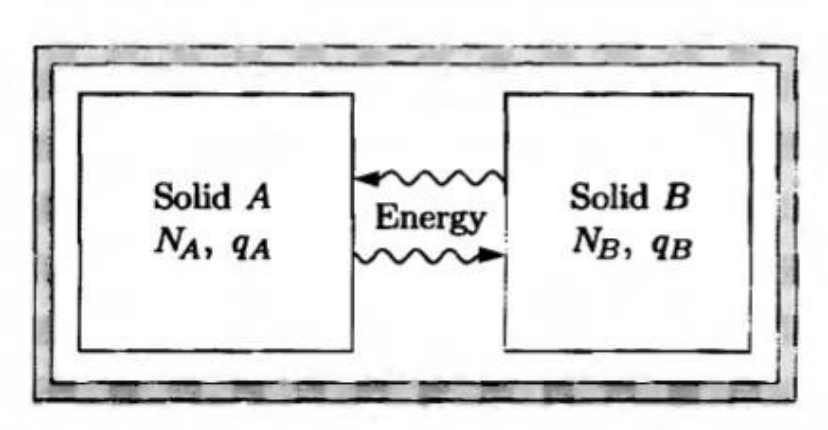
\includegraphics[width=6cm]{figure11.png}
    \caption{Two Einstein solids that can exchange energy with each other, isolated from the rest of the universe.}
\label{fig:two-einstein-solids}
\end{figure}\\
\hspace*{10mm}Now, suppose that each solid, $A$ and $B$, contains three harmonic oscillators and they contain a total of six units of energy:
\begin{equation}\tag{2.10}
N_A = N_B = 3;\quad q_{\text{total}}=q_A+q_B=6
\end{equation}
where $q$ denotes the number of units of energy and the energy $U$ is given by $U=qhf$. There are seven possible macrostates, with $q_A=0,1,\dots,6$. The total multiplicity of any macrostate, $\Omega_{\text{total}}$, is the product of the individual multiplicities, since the systems are independent of each other: For each of the $\Omega_A$ microstates available to solid $A$, there are $\Omega_B$ microstates available to solid $B$. Over long time scales, the number of microstates accessible to the system is 462, the number obtained by applying the standard formula to the entire system of six oscillators and six energy units. \\
\hspace*{10mm}Furthermore, assume that over long time scales, the energy gets passed around randomly in such a way that all 462 microstates are equally probable. This assumption is called the fundamental assumption of statistical mechanics. The fundamental assumption of statistical mechanics states that in an isolated system in thermal equilibrium, all accessible microstates are equally probable.\\
\hspace*{10mm}Invoking the fundamental assumption for the two Einstein solid system, we can conclude that, although all 462 microstates are equally probable, some macrostates are more probable than others. The chance of finding the system in the fourth macrostate (with three energy units in each solid) is 100/462, while the chance of finding it in the first macrostate (with all the energy in solid $B$) is only 28/462. If all the energy is in solid $B$ initially, it is likely that the energy will distribute later on.\\
\hspace*{10mm}Heat is a probabilistic phenomenon, not absolutely certain, but extremely likely. The spontaneous flow of energy stops when a system is at, or very near, its most likely macrostate, that is the macrostate with the greatest multiplicity. This law of increase of multiplicity is also known as the second law of thermodynamics. 
\newpage
\subsection{Large Systems}
For a system of two interacting Einstein solids, as the number of oscillators each solid contains increases, the multiplicity function becomes sharper (see Figure 12). 
\begin{figure}[htp]
    \centering
    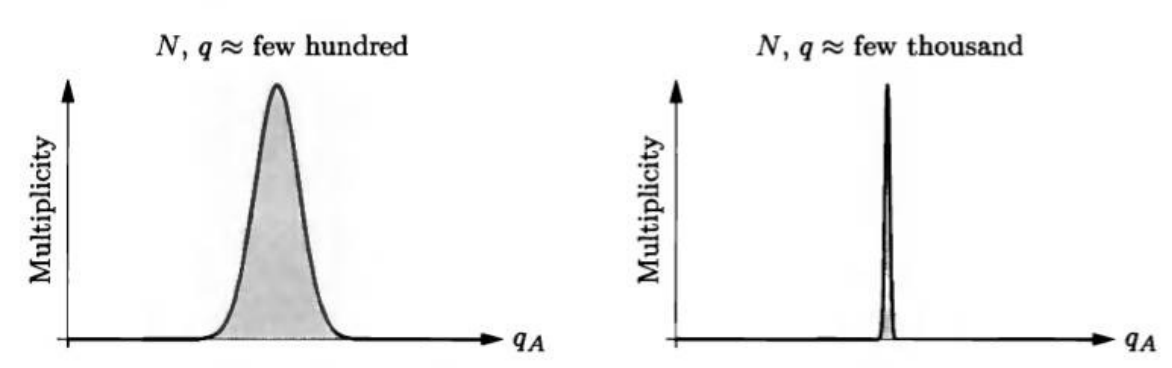
\includegraphics[width=6cm]{figure12.png}
    \caption{Typical multiplicity graphs for two interacting Einstein solids, containing a few hundred oscillators and energy units (left) and a few thousand (right). As the size of the system increases, the preak becomes very narrow relative to the full horizontal scale. For $N\approx q\approx 10^{20}$, the peak is too sharp to draw.}
\label{fig:large-systems}
\end{figure}
\subsubsection*{Very Large Numbers}
There are three kinds of numbers that commonly occur in statistical mechanics: small numbers, large numbers, and very large numbers.\\
\hspace*{10mm}Small numbers are small numbers. \\
\hspace*{10mm}Large numbers are much larger than small numbers, and are frequently made by exponentiating small numbers. The most important property of large numbers is that a small number can be added to a large number without changing it. The only expectation to this rule is when the same large number is subtracted off.\\
\hspace*{10mm}Very large numbers are even larger than large numbers, and can be made by exponentiating large numbers. Very large numbers have the property that they can multiplied by large numbers without changing them. The only exception is when the product is divided by the same very large number. 
\subsubsection*{Stirling's Approximation}
Stirlings's approximation can be used to evaluate factorials of large numbers: 
\begin{equation}\tag{2.14}
N!\approx N^N e^{-N}\sqrt{2\pi N}.
\end{equation}
This approximation is accurate in the limit where $N\gg1$. \\
\hspace*{10mm}The quantity $N!$ is the product of $N$ factors, from 1 up to $N$. A crude approximation would be to replace each of the $N$ factors in the factorial by $N$ so $N!\approx N^N$. This is a gross overestimate, on average, each factor is smaller by a factor of $e$:
\begin{equation}\tag{2.15}
    N!\approx \left(\frac{N}{e}\right)^N = N^Ne^{-N}.
\end{equation}
Although this values is still of by a factor of $\sqrt{2\pi N}$, if $N$ is a large number then $N!$ is a very large number and the correction factor can be omitted. Equation 2.15, can also be written as 
\begin{equation}\tag{2.16}
    \ln{N!}\approx N\ln{N} - N.
\end{equation}
\newpage
\subsubsection*{Multiplicity of a Large Einstein Solid}
Consider the case $q\gg N$, when there are more energy units than oscillators. As such, we have 
\begin{equation}\tag{2.17}
\Omega(N, q)=\binom{q+N-1}{q} = \frac{(q+N-1)!}{q!(N-1)!}\approx \frac{(q+N)!}{q!N!}
\end{equation}
where the last approximation is made since the difference between $N!$ and $(N-1)!$ factorial is only a large factor $N$ which is insignificant in a very large number like $\Omega$. Then, taking the natural logarithm and applying Stirling's approximation in the form 2.16:
\begin{align*}
\ln{\Omega}&=\ln{\left(\frac{(q+N)!}{q!N!}\right)}\\
&= \ln{(q+N)!}-\ln{q!}-\ln{N!}\\
&\approx (q+N)\ln{(q+N)}-(q+N)-q\ln{q}+q-N\ln{N}+N\\
&= (q+N)\ln{(q+N)}-q\ln{q}-N\ln{N}. 
\end{align*}
Manipulating the first logarithm using the Taylor expansion of the logarithm, $\ln{(1+x)}\approx x$ for $|x|\ll 1$, we obtain 
\begin{align*}\tag{2.19}
\ln{(q+N)}&= \ln{\left[q\left(1+\frac{N}{q}\right)\right]}\\
&= \ln{q} + \ln{\left(1+\frac{N}{q}\right)}\\
&\approx \ln{q} +\frac{N}{q}.
\end{align*}
Substituting equation 2.19 into equation 2.18, we obtain 
\begin{equation}\tag{2.20}
\ln{\Omega} \approx N\ln{\frac{q}{N}}+\frac{N^2}{q}.   
\end{equation}
Since the last term becomes negligible in the limit $q\gg N$, exponentiating the first two terms gives 
\begin{equation}\tag{2.21}
\Omega(N, q)\approx e^{N\ln{(q/N)}}e^N=\left(\frac{eq}{N}\right)^N\quad\text{(when $q\gg N$).}  
\end{equation}
The exponent is a large number, so $\Omega$ is a very large number. Furthermore, $\Omega$ will increase by a lot if $N$ or $q$ is increased slightly, due to the large exponent. 
\newpage
\subsubsection*{Sharpness of the Multiplicity Function}
To find how skinny the peak of a multiplicity function of two large interacting Einstein solids is, first assume that each solid has $N$ oscillators, denote the total number of energy units as $q$, and assume that $q$ is much larger than $N$, so equation 2.21 may be used. Then,the multiplicity of the combined system, for any given macrostate, is 
\begin{equation}\tag{2.22}
\Omega = \left(\frac{eq_A}{N}\right)^N\left(\frac{eq_B}{N}\right)^N  = \left(\frac{e}{N}\right)^{2N}(q_Aq_B)^N,
\end{equation}
where $q_A$ and $q_B$ are the numbers of energy units in solids $A$ and $B$. (Note that $q_A +q_B$ must equal $q$.)\\
\hspace*{10mm}As a function of $q_A$, equation 2.22 has a very sharp peak at $q_A = q/2$, where the energy is distributed equally between the solids. The height of the peak is a very large number:
\begin{equation}\tag{2.23}
\Omega_{\text{max}}=\left(\frac{e}{N}\right)^{2N}\left(\frac{q}{2}\right)^{2N}    
\end{equation}
To determine the properties of the graph near this peak, let 
\begin{equation}\tag{2.24}
q_A=\frac{q}{2}+x,\quad q_B=\frac{q}{2}-x,
\end{equation}
where $x$ is any number smaller than q (but still possiblly large). Substituting expression 2.24 into equation 2.22, we have
\begin{equation}\tag{2.25}
\Omega = \left(\frac{e}{N}\right)^{2N}\left[\left(\frac{q}{2}\right)-x^2\right]^N.
\end{equation}
Then simplifying the second factor as was done in equation 2.19
\begin{equation}\tag{2.26}
\ln{\left[\left(\frac{q}{2}\right)-x^2\right]^N} \approx N\left[\ln{\left(\frac{q}{2}\right)^2}-\left(\frac{2x}{q}\right)^2\right].
\end{equation}
Exponentiating the last expression and substituting into equation 2.25, 
\begin{equation}\tag{2.27}
\Omega = \left(\frac{e}{N}\right)^{2N}e^{N\ln{(q/2)}^2}e^{-N(2x/q)^2}=\Omega_{\text{max}}\cdot e^{-N(2x/q)^2}.
\end{equation}
A function of this form is called a Gaussian; it has a peak at $x=0$ and a sharp fall-off on either side, as shown in Figure 13. The multiplicity falls off to $1/e$ of its maximum value when 
\begin{equation}
N\left(\frac{2x}{q}\right)^2 =1\quad\text{or}\quad x=\frac{q}{2\sqrt{N}}.  
\end{equation}
\hspace*{10mm}When two large Einstein solids are in thermal equilibrium with each other, any random fluctuations away from the most likely macrostate will be unmeasurable. Once the system has had time to come to thermal equilibrium, so that all microstates are equally probable, it will be in its most likely macrostate. The limit where a system becomes infinitely large, so that fluctuations away from the most likely macrostate never occur, is called the thermodynamic limit. 
\newpage
\begin{figure}[htp]
    \centering
    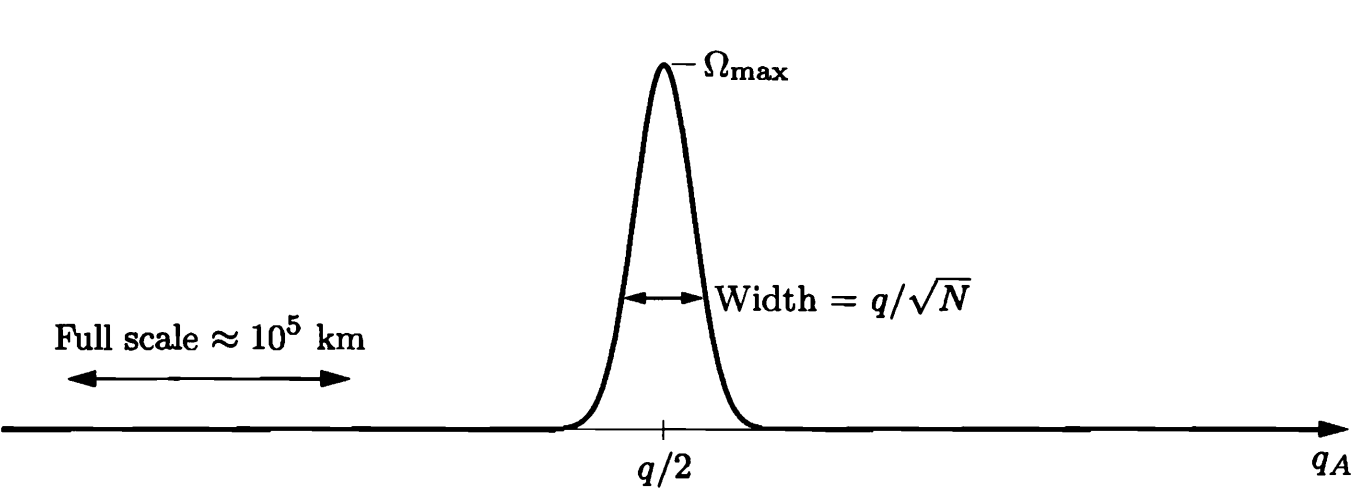
\includegraphics[width=6cm]{figure13.png}
    \caption{Multiplicity of a system of two large Einstein solids with many energy units per oscillator (high-temperature limit). Only a tiny fraction of the full horizontal scale is shown.}
\label{fig:two-einstein-multiplicity}
\end{figure}
\newpage 
\subsection{The Ideal Gas}
For any pair of interacting objects, only a tiny fraction of the macrostates of the large interacting system have reasonably large probabilities, provided that the number of particles and the number of energy units are both large.\\
\hspace*{10mm}The multiplicity of an ideal gas depends on its volume as well as its total energy and number of particles. Furthermore, when two gases interact, they can often expand and contract, and exchange molecules, in addition to exchanging energy.
\newpage
\subsubsection*{Multiplicity of a Monatomic Ideal Gas}
Suppose we have a single monatomic ideal gas atom, with total energy $U$, in a container of volume $V$. To determine the multiplicity of this system, first note that since a container with twice the volume offers twice as many states to a molecule, the multiplicity should be proportional to $V$. Also, the more different momentum vectors the molecule has, the more states are available, so the multiplicity should also be proportional to the volume of available momentum space. (Momentum space is an imaginary space in which the axes are $p_x$, $p_y$, and $p_z$. Each point in momentum space corresponds to a momentum vector for the particle.) So, we have 
\begin{equation}\tag{2.29}
\Omega_1 \propto V\cdot V_p, 
\end{equation}
where $V$ is the volume of ordinary space (or position space), and $V_p$ is the volume of momentum space, and the 1 subscript indicates that this is for a gas of just one molecule.\\
\hspace*{10mm}To determine the available volume of momentum space, $V_p$, observe that since the molecule's kinetic energy must equal $U$, there is a constraint:
\begin{equation}\tag{2.30}
U=\frac{1}{2}m(v_x^2+v_y^2+v_z^2)=\frac{1}{2m}(p_x^2+p_y^2+p_z^2)    
\end{equation}
or equivalently 
\begin{equation}\tag{2.31}
p_x^2+p_y^2+p_z^2 = 2mU    
\end{equation}
which defines the surface of a sphere in momentum space with radius $\sqrt{2mU}$ (see Figure 14). The volume of momentum space is the surface area of this sphere (perhaps multiplied by a small thickness if $U$ is allowed to fluctuate somewhat.)
\begin{figure}[htp]
    \centering
    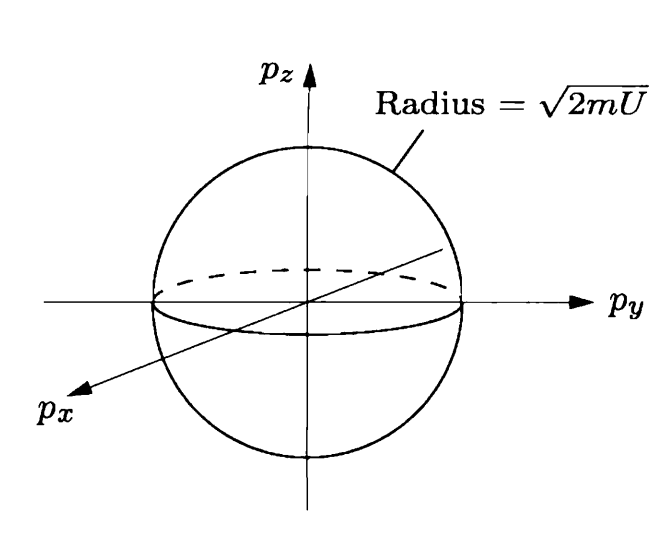
\includegraphics[width=6cm]{figure14.png}
    \caption{A sphere in momentum space with radius $\sqrt{2mU}$. If a molecule has energy $U$, its momentum space vector must lie somewhere on the surface of this sphere.}
\label{fig:momentum-space-volume}
\end{figure}\\
To count the number of microstates, we must invoke quantum mechanics. In quantum mechanics, the state of a system is described by a wavefunction, which is spread out in both position space and momentum space. The less spread out the wavefunction is in position space, the more spread out it must be momentum space, and vice versa. This is the Heisenberg uncertainty principle:
\begin{equation}\tag{2.32}
(\Delta x)(\Delta p_x) \approx h,
\end{equation}
where $\Delta x$ is spread in $x$, $\Delta p_x$ is the spread in $p_x$, and $h$ is Plank's constant. (The product of $\Delta x$ and $\Delta p_x$ can also be more than $h$.) The same limitation applies to $y$ and $p_y$, and to $z$ and $p_z$.\\
\hspace*{10mm}Although the number of allowed wavefunctions in quantum mechanics is infinite, the number of independent wavefunctions is finite, if the total available position space and momentum space are limited. In the one-dimensional example shown in Figure 15, the number of distinct position states is $L/(\Delta x)$, while the number of distinct momentum states is $L_p/(\Delta p_x)$.
\begin{figure}[htp]
    \centering
    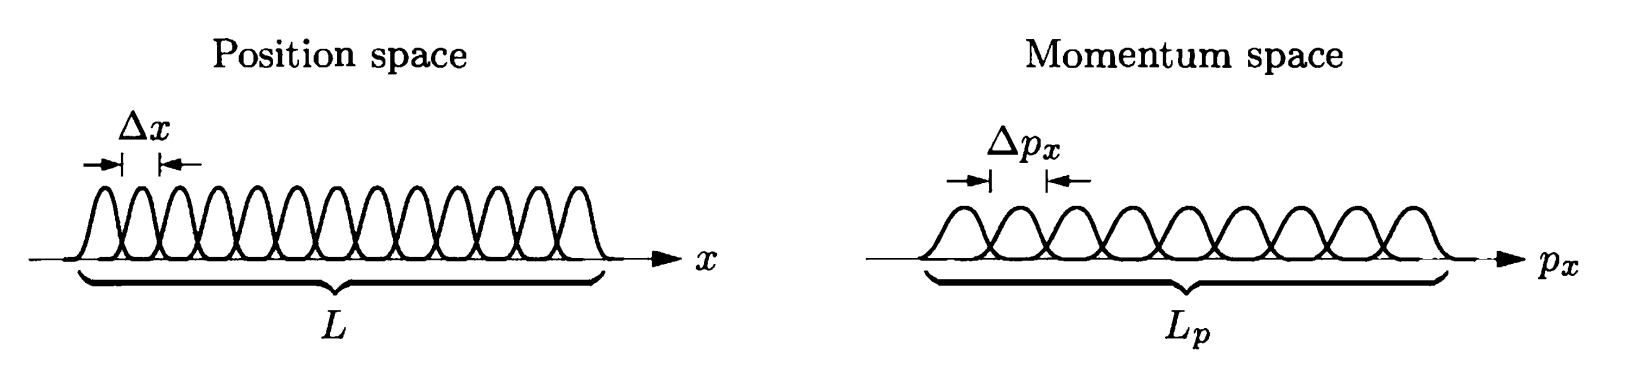
\includegraphics[width=6cm]{figure15.png}
    \caption{A number of independent position states and momentum states for a quantum-mechanical particle moving in one dimension. If we make the wavefunctions narrower in position space, they become wider in momentum space, and vice versa.}
\label{fig:momentum-position-space}
\end{figure}\\
The total number of distinct states is the product, 
\begin{equation}\tag{2.33}
\frac{L}{\Delta x}\frac{L_p}{\Delta p_x}=\frac{LL_p}{h},    
\end{equation}
according to the uncertainty principle. In three dimensions, the lengths become volumes and there are three factors of $h$:
\begin{equation}\tag{2.34}
\Omega_1 = \frac{VV_p}{h^3}.    
\end{equation}
\hspace*{19mm}If a second molecule is added, factors of the form of equation 2.34 for each molecule must be multiplied together because for each state of state of molecule 1, there are $\Omega_1$ states for molecule 2. However this is not quite true as the $V_p$ factors are  more complicated, since only the total energy of the two molecules is constrained. As such, equation 2.31 becomes 
\begin{equation}\tag{2.35}
p_{1x}^2+p_{1y}^2+p_{1z}^2+p_{2x}^2+p_{2y}^2+p_{2z}^2 = 2mU,    
\end{equation}
assuming that both molecules have the same mass. This equation defines the surface of a six-dimensional hypersphere in six-dimensional momentum space. \\
\hspace*{10mm}So the multiplicity function for an ideal gas of two molecules is
\begin{equation}\tag{2.36}
\Omega_2=\frac{V^2}{h^6}\times \text{(area of momentum hypersphere)}.
\end{equation}
This formulas is correct only if the two molecules are distinguishable from each other. If they're indistinguishable, then the microstates have been overcounted by a factor of 2, since interchanging the molecules with each other does not produce a distinct state (see Figure 16). Thus the multiplicity for a gas of two indistinguishable molecules is 
\begin{equation}\tag{2.37}
\Omega_2 = \frac{1}{2}\frac{V^2}{h^6}\times \text{(area of momentum hypersphere)}.
\end{equation}
\begin{figure}[htp]
    \centering
    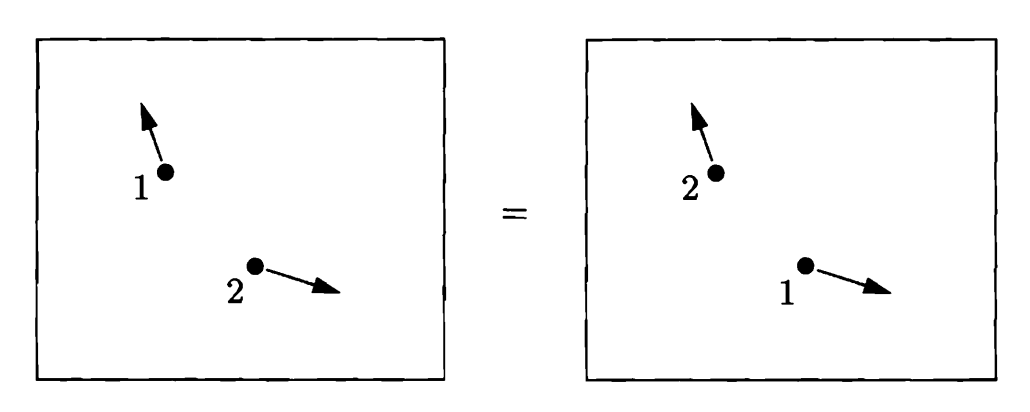
\includegraphics[width=6cm]{figure16.png}
    \caption{In a gas of two identical molecules, interchanging the states of the molecules leaves the system in the same state as before.}
\label{fig:identitical-molecules}
\end{figure}
\newpage
\hspace*{10mm}For an ideal gas of $N$ indistinguishable molecules, the multiplicity function contains $N$ factors of $V$, divided by $3N$ factors of $h$. The factor that compensates for the overcounting is $1/N!$, the number of ways of interchanging the molecules and the momentum-space factor is the surface area of a $3N$-dimensional hypersphere whose radius is $\sqrt{2mU}$:
\begin{equation}\tag{2.38}
\Omega_N = \frac{1}{N!}\frac{V^N}{h^{3N}}\times \text{(area of momentum hypersphere)}.  
\end{equation}
\hspace*{10mm}For a general $d$-dimensional hypersphere of radius $r$, the surface area is given by 
\begin{equation}\tag{2.39}
\text{"area"}=\frac{2\pi^{d/2}}{\left(\frac{d}{2}-1\right)!}r^{d-1}.
\end{equation}
\hspace*{10mm}Substituting equation 2.39 (with $d=3N$ and $r=\sqrt{2mU}$) into equation 2.38, we have
\begin{equation}\tag{2.40}
\Omega_N = \frac{1}{N!}\frac{V^N}{h^{3N}}\frac{2\pi^{3N/2}}{\left(\frac{3N}{2}-1\right)!}(\sqrt{2mU})^{3N-1}\approx \frac{1}{N!}\frac{V^N}{h^{3N}}\frac{\pi^{3N/2}}{(3N/2)!}(\sqrt{2mU})^{3N}. 
\end{equation}
\hspace*{10mm}Furthermore, by equation 2.40, the multiplicity of a monatomic ideal gas has a dependence on $U$ and $V$ by the following relation
\begin{equation}\tag{2.41}
\Omega(U,V,N)=f(N)V^N U^{3N/2}
\end{equation}
where $f(N)$ is a complicated function of $N$.\\
\hspace*{10mm}Note that the exponent on $U$ in formula 2.41 is $1/2$ times the total number of degrees of freedom ($3N$) in the monatomic gas. The same is true of the multiplicity of an Einstein solid in the high-temperature limit, equation 2.21. These results are special cases of a more general theorem: For any system with only quadratic degrees of freedom, having so many units of energy that energy quantization is unnoticeable, the multiplicity is proportional to $U^{Nf/2}$, where $Nf$ is the total number of degrees of freedom.
\newpage
\subsubsection*{Interacting Ideal Gases}
Suppose that two ideal gases are separated by a partition that allows energy to pass through (see Figure 17). If each gas has $N$ molecules (of the same species), then the multiplicity of this system is 
\begin{equation}\tag{2.42}
\Omega_{\text{total}}=|f(N)|^2(V_AV_B)^N(U_AU_B)^{3N/2}.    
\end{equation}
This expression essentially has the same form as the corresponding result for a pair of Einstein solids (equation 2.22): Both energies are raised to a large exponent. As such, the multiplicity function plotted as a function of $U_A$, has a very sharp peak:
\begin{equation}\tag{2.43}
\text{width of peak}=\frac{U_{\text{total}}}{\sqrt{3N/2}}. 
\end{equation}
Provided that $N$ is large, only a tiny fraction of the macrostates have a reasonable chance of occurring, assuming that the system is in equilibrium. 
\begin{figure}[htp]
    \centering
    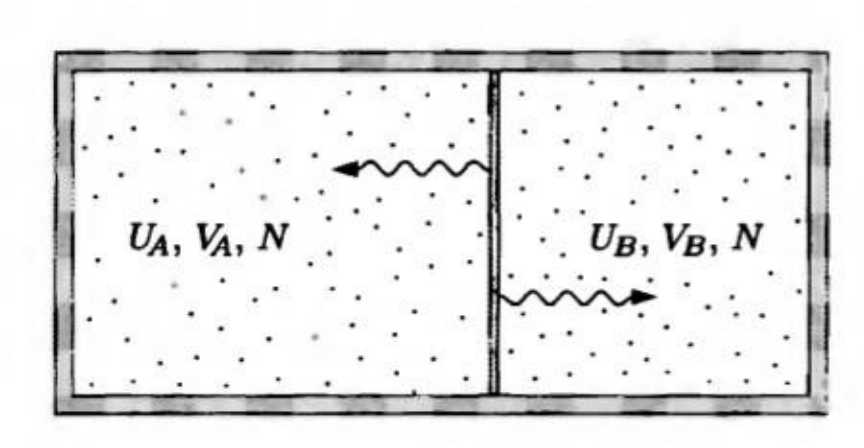
\includegraphics[width=6cm]{figure17.png}
    \caption{Two ideal gases, each confined to a fixed volume, separated by a partition that allows energy to pass through. The total energy of the gases is fixed.}
\label{fig:identitical-molecules}
\end{figure}\\
\hspace*{10mm}In addition to exchanging energy, the gases could exchange volume; that is, the partition can move back and forth, as one gas expands and the other is compressed. The argument applied to energy can be applied to volume, so the multiplicity, plotted as a function of $V_A$, again has a very sharp peak:
\begin{equation}\tag{2.44}
\text{width of peak}=\frac{V_{\text{total}}}{\sqrt{N}}. 
\end{equation}
So the equilibrium macrostate is essentially determined, to within a fraction of the total volume available (if $N$ is large). 
\begin{figure}[htp]
    \centering
    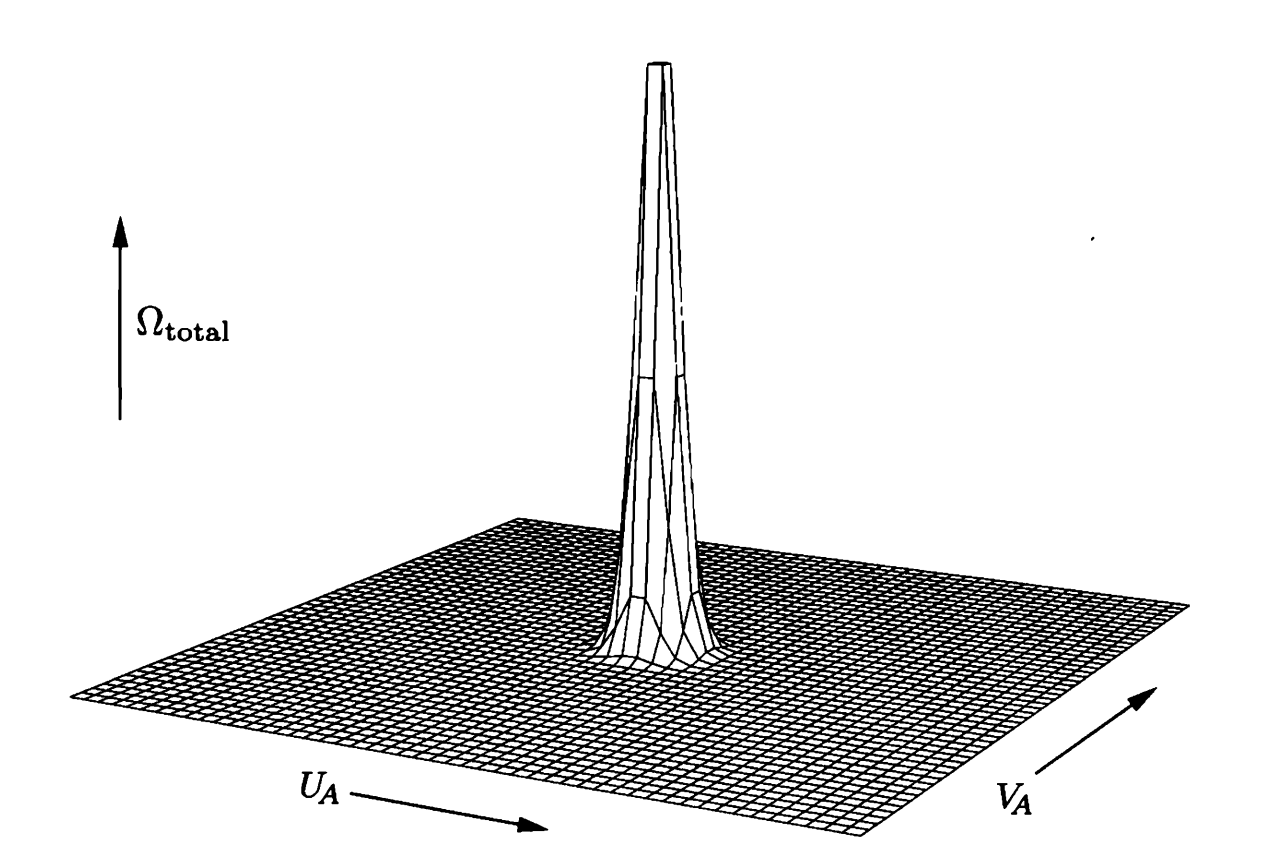
\includegraphics[width=6cm]{figure18.png}
    \caption{Multiplicity of a system of two ideal gases, as a function of the energy and volume of gas $A$ (with the total energy and total volume held fixed). If the number of molecules in each gas is large, the full horizontal scale would stretch far beyond the edge of the page.}
\label{fig:3d-plot}
\end{figure}
\subsection{Entropy}
For any system that contains enough particles and units of energy for the statistics of very large numbers to apply: Any large system in equilibrium will be found in the macrostate with the greatest multiplicity (aside from fluctuations that are normally too small to measure). This is a more general statement of the second law of thermodynamics. Another way to say it is: Multiplicity tends to increase.\\
\hspace*{10mm}Since multiplicities tend to be very large numbers, it is convenient to work with the natural logarithm of the multiplicity instead of the multiplicity itself. The natural logarithm of the multiplicity multiplied by a factor of Boltzmann's constant gives us the entropy, denoted $S$:\
\begin{equation}\tag{2.45}
    S\equiv k\ln{\Omega}
\end{equation}
In words, entropy is the logarithm of the number of ways of arranging things in a system times Boltzmann's constant. The logarithm turns a very large number, the multiplicity, into an ordinary large number. Entropy, $S$ has units of energy divided by temperature, or J/K in the SI system.\\
\hspace*{10mm}Consider a large Einstein solid with $N$ oscillators, $q$ units of energy and $q\gg N$. Since $\Omega =(eq/N)^N$, 
\begin{equation}\tag{2.46}
S=k\ln{(eq/N)^N}=Nk[\ln{(q/N)}+1].    
\end{equation}
Notice that increasing either $q$ or $N$ increases the entropy of an Einstein solid (though not in direct proportion).\\
\hspace*{10mm}Generally, the more particles that in a system, and the more energy it contains, the greater its multiplicity and its entropy. Besides adding particles and energy, the entropy of a system can be increased by letting it expand into a larger space, or breaking large molecules apart into small ones, or mixing together substances that were once separate. In each of these cases, the total number of possible arrangements increases.\\
\hspace*{10mm}The total entropy of a composite system is the sum of the entropies of its parts. If there are two parts, $A$ and $B$, then 
\begin{equation}\tag{2.48}
S_{\text{total}}=k\ln{\Omega_{\text{total}}}=k\ln{(\Omega_A\Omega_B)}=k\ln{\Omega_A}+k\ln{\Omega_B}=S_A+S_B    
\end{equation}
where the macrostates of systems $A$ and $B$ are specified separately. If these systems interact, then those macrostates can fluctuate over time, and to compute the entropy over long time scales we should compute $\Omega_{\text{total}}$ by summing over all macrostates for the two systems. Entropy, like multiplicity, is a function of the number of accessible microstates, and this number depends on the time scale under consideration. However, in practice, this distinction rarely matters. If we assume that the composite system is in its most likely macrostate, we get the same entropy as if we sum over all macrostates.\\
\hspace*{10mm}Since the natural logarithm is a monotonically increasing function of its argument, a macrostate with higher multiplicity also has higher entropy. Therefore the second law of thermodynamics may be stated as follows: Any large system in equilibrium will be found in the macrostate with the greatest entropy (aside from fluctuations that are normally too small to measure). Or more briefly: Entropy tends to increase. Note, however, that a graph of entropy versus some variable (such as $U_A$ or $V_A$) that is allowed to fluctuate will generally not have a sharp peak. Taking the logarithm smooths out the peak that was present in the multiplicity function. This does not affect the fact that fluctuations away from the macrostate of greatest entropy will be negligible for any reasonably large system.\\
\hspace*{10mm}Spontaneous processes always occur because of a net increase in entropy. If entropy is decreased in one place, at least as much entropy is created somewhere else. 
\subsubsection*{Entropy of an Ideal Gas}
The formula for the entropy of a monatomic ideal gas known as the Sackur-Tetrode equation is given by
\begin{equation}\tag{2.49}
S=Nk\left[\ln{\left(\frac{V}{N}\left(\frac{4\pi mU}{3nh^2}\right)^{3/2}\right)}+\frac{5}{2}\right].
\end{equation}
\hspace*{10mm}The entropy of an ideal gas depends on its volume, energy, and number of particles. Increasing any of these three variables increases the entropy. The simplest dependence is on the volume; for instance, if the volume changes from $V_i$ to $V_f$ while $U$ and $N$ are held fixed, the entropy changes by 
\begin{equation}
\Delta S = Nk\ln{\frac{V_f}{V_i}}\quad\text{($U, N$ fixed).}
\end{equation}
This formula applies, for instance, to a quasistatic isothermal expansion where the gas pushes on a piston, doing mechanical work, while heat is simultaneously supplied from outside to keep the gas at constant temperature. In this case, the heat input causes the entropy to increase. Putting heat into a system always increases is entropy.\\
\hspace*{10mm}Consider the process shown in Figure 19. Initially, the gas is separated by a partition from an evacuated chamber. The partition is then punctured, letting the gas freely expand to fill the whole available space. This process is called free expansion. Since the gas isn't pushing on anything, no work is done. Furthermore, no heat flows into or out of the gas. Therefore, by the first law of thermodynamics, 
\begin{equation}\tag{2.52}
\Delta U=Q+W=0+0=0.    
\end{equation}
The energy content of the gas does not change during free expansion, hence formula 2.51 applies. However, the entropy increase was not caused by the input of heat; instead new entropy was manufactured. 
\begin{figure}[htp]
    \centering
    \includegraphics[width=6cm]{figure19.png}
    \caption{Free expansion of a gas into a vacuum. Because the gas neither does work nor absorbs heat, its energy is unchanged. The entropy of the gas increases, however.}
\label{fig:momentum-space-volume}
\end{figure}\\
\newpage
\subsubsection*{Entropy of Mixing}
Entropy can be created by letting two different materials mix each other. Suppose we have two different monatomic ideal gases, $A$ and $B$, each with the same energy, volume, and number of particles. They occupy the two halves of a divided chamber, separated by a partition (see Figure 20). If the partition is removed, the entropy increases. To calculate by how much, we can treat each gas as a separate system, even after they mix. Since gas $A$ expands to fill twice its initial volume, its entropy increases by 
\begin{equation}\tag{2.58}
\Delta S_A = Nk\ln{\frac{V_f}{V_i}}=Nk\ln{2},    
\end{equation}
while the entropy of gas $B$ increases by the same amount, giving a total increase of 
\begin{equation}\tag{2.54}
\Delta S_\text{total} = \Delta_A + \Delta_B = 2Nk\ln{2}. 
\end{equation}
This increase is called the entropy of mixing. 
\begin{figure}[htp]
    \centering
    \includegraphics[width=6cm]{figure20.png}
    \caption{Two different gases, separated by a partition. When the partition is removed, each gas expands to fill the whole container, mixing with the other and creating entropy.}
\label{fig:momentum-space-volume}
\end{figure}\\
\hspace*{10mm}This result applies only if the two gases are different. If we start with the same gas on both sides, the entropy doesn't increase at all when the partition is removed. (The total multiplicity increases, because the distribution of molecules between the two sides can now fluctuate. But the multiplicity increases only by a large factor, which has negligible effect on the entropy.)\\
\hspace*{10mm}Suppose we start with a mole of helium in the chamber without a partition. Its total entropy is given by the Sackur-Tetrode equation, equation 2.49. If a mole of argon with the same thermal energy $U$ is added, the entropy approximately doubles:
\begin{equation}\tag{2.56}
S_\text{total}=S_\text{helium} + S_\text{argon}.    
\end{equation}
(Because equation 2.49 has a molecular mass term, the entropy of the argon is somewhat greater than the entropy of the helium.) However, if a second mole of helium is added, the entropy does not double. If the values of both $N$ and $U$ are doubled in equation 2.49, the ratio $U/N$ inside the logarithm is unchanged and the $N$ out front becomes $2N$. But since there is another $N$ inside the logarithm which also becomes $2N$, the total entropy is less by a term of $2Nk\ln{2}$, the entropy of mixing.\\
\hspace*{10mm}Gibbs paradox concerns the issues that would arise if molecules in a gas were distinguishable. Namely, partitioning a tank of a monatomic ideal gas like helium would violate the second law of thermodynamics as each half would have significantly less than half of the original entropy. The best resolution of the paradox is to assume that all atoms of a given type are indistinguishable. 
\newpage
\subsubsection*{Reversible and Irreversible Processes}
If a physical process increases the total entropy of the universe, that process cannot happen in reverse, since this would violate the second law of thermodynamics. Processes that create new entropy are therefore said to be irreversible. A process that leaves the total entropy of the universe unchanged is reversible. In practice, no macroscopic process is perfectly reversible, although some processes come close enough for most purposes.\\
\hspace*{10mm}The very sudden expansion of a system, for instance, the free expansion of a gas, creates new entropy. A gradual compression or expansion does not by itself change the entropy of a system. Any reversible volume change must be quasistatic, so that $W=-P\Delta V$. (A quasistatic process can be irreversible if there is also heat flowing in or out or if entropy is being created in some other way.)\\
\hspace*{10mm}To understand why the slow compression of a gas does not cause its entropy to increase, suppose that the molecules in the gas inhabit various quantum-mechanical wavefunctions, each filling the entire box, with discrete (though very closed spaced) energy levels. When the gas is compressed, each wavefunction gets squeezed, so the energies of all the levels increase, and each molecule's energy increases accordingly, But if the compression is sufficiently slow, molecules will not be kicked up into higher energy levels; a molecule that starts in the $n$th level remains in the $n$th level (although the energy of that level increases). Thus the number of ways of arranging the molecules among the various energy levels remains the same, that is, the multiplicity and entropy do not change. If the compression is violent enough to kick molecules up into higher levels, then the number of possible arrangements will increase and so will the entropy.\\
\hspace*{10mm}The flow of heat from a hot object to a cold one occurs because the total multiplicity of the combined system increases, hence the total entropy increases also, and heat flow is always irreversible. The increase in entropy becomes negligible in the limit where the temperature difference between the two objects goes to zero. Reversible heat flow refers to very slow heat flow, between objects that are nearly the same temperature. In the reversible limit, changing the temperature of one of the objects only infinitesimally can cause the heat to flow in the opposite direction. Similarly, during a quasistatic volume change, an infinitesimal change in the pressure will reverse the direction. Thus, a reversible process can be defined as one that can be reversed by changing the conditions only infinitesimally. 
\newpage
\section{Interactions and Implications}
\subsection{Temperature}
The second law says that when two objects are in thermal equilibrium, their total entropy has reached its maximum possible value.\\
\hspace*{10mm}Consider two Einstein solids, $A$ and $B$, that are weakly coupled so that they can exchange energy (but with the total energy fixed). Suppose that the numbers of oscillators in the two solids are $N_A=300$ and $N_B=200$, and that they are sharing 100 units of energy: $q_\text{total}=100$. Table 2 lists the various macrostates, their multiplicities, columns for the entropy of solid $A$, the entropy of solid $B$, and the total entropy (which can be obtained either by adding $S_A$ and $S_B$, or by taking the logarithm of $\Omega_\text{total}$).\\
\begin{table}[htp]
\centering
\begin{tabular}{ccc|ccc|cc}
$q_A$ & $\Omega_A$ & $S_A/k$ & $q_B$ & $\Omega_B$ & $S_B/k$ & $\Omega_\text{total}$ & $S_\text{total}/k$\\
\hline
0 & 1 & 0 & 100 & \num{2.8e81} & 187.5 & \num{2.8e81} & 187.5 \\
1 & 300 & 5.7 & 99 & \num{9.3e80} & 186.4 & \num{2.8e83} & \num{192.1}\\
2 & 45150 & 10.7 & 98 & \num{3.1e80} & 185.3 & \num{1.4e85} & 196.0\\
\vdots & \vdots & \vdots & \vdots & \vdots & \vdots & \vdots & \vdots\\
11 & \num{5.3e19} & 45.4 & 89 & \num{1.1e76} & 175.1 & \num{5.9e95} & 220.5 \\
12 & \num{1.4e21} & 48.7 & 88 & \num{3.4e75} & 173.9 & \num{4.7e96} & \num{222.6}\\
13 & \num{3.3e22} & 51.9 & 87 & \num{1.0e75} & 172.7 & \num{3.5e97} & 224.6\\
\vdots & \vdots & \vdots & \vdots & \vdots & \vdots & \vdots & \vdots\\
59 & \num{2.2e68} & 157.4 & 41 & \num{3.1e46} & 107.0 & \num{6.8e114} & 264.4 \\
60 & \num{1.3e69} & 159.1 & 40 & \num{5.3e45} & 105.5 & \num{6.9e114} & \num{264.4}\\
61 & \num{7.7e69} & 160.9 & 39 & \num{8.8e44} & 103.5 & \num{6.8e114} & 264.4\\
\vdots & \vdots & \vdots & \vdots & \vdots & \vdots & \vdots & \vdots\\
100 & \num{1.7e96} & \num{221.6} & 0 & 1 & 0 & \num{1.7e96} & 221.6
\end{tabular}
\caption{Macrostates, multiplicities, and entropies of a system of two Einstein solids, one with 300 oscillators and ther with 200, sharing a total of 100 units of energy.}
\label{tab:microstates_macrostates}
\end{table}\\
Figure 22 shows a graph of $S_A$, $S_B$, and $S_\text{total}$ (in units of Boltzmann's constant), for the same parameters as in the table. The equilibrium point is at $q_A=60$, where $S_\text{total}$ reaches its maximum value. At this point, the tangent to the graph of $S_\text{total}$ is horizontal ; that is, 
\begin{equation}\tag{3.1}
\frac{\partial S_\text{total}}{\partial q_A}=0\quad\text{or}\quad\frac{\partial S_\text{total}}{\partial U_A}=0\quad\text{at equilibrium.}
\end{equation}
Since the slope of the $S_\text{total}$ graph is the sum of the slopes of the $S_A$ and $S_B$ graphs, 
\begin{equation}\tag{3.2}
\frac{\partial S_A}{\partial U_A}+\frac{\partial S_B}{\partial U_A}=0\quad\text{at equilibrium.} 
\end{equation}
Since $dU_A = -dU_B$, 
\begin{equation}\tag{3.3}
\frac{\partial S_A}{\partial U_A}=\frac{\partial S_B}{\partial U_B} \quad\text{at equilibrium.}
\end{equation}
When both systems are in equilibrium, the slope of their entropy vs. energy graphs are the same.\\
\hspace*{10mm}By the second law, energy will always tend to flow into the object with the steeper $S$ vs. $U$ graph, and out of the object with the shallower $S$ vs. $U$ graph. The former wants to gain energy (in order to increase its entropy), while the latter doesn't mind losing a bit of energy (since its entropy doesn't decrease by much). A steep slope must correspond to a low temperature, while a shallow slope must correspond to a higher temperature.\\
\begin{figure}[htp]
    \centering
    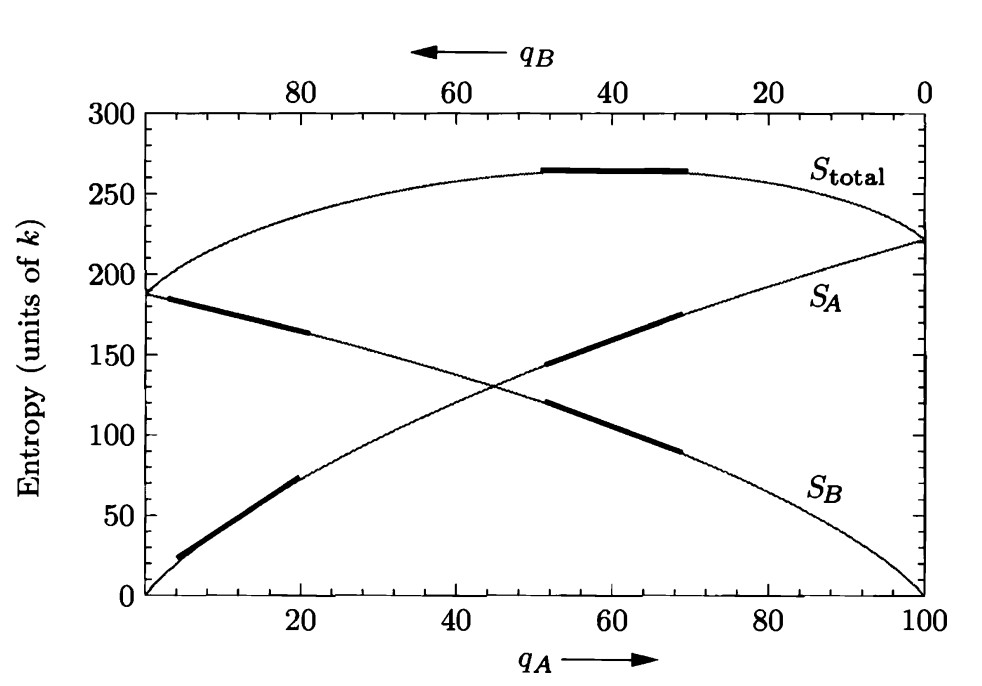
\includegraphics[width=6cm]{figure22.png}
    \caption{A plot of the entropies calculated in Table 2. At equilibrium ($q_A=60$}, the total entropy is a maximum so its graph has a horizontal tangent; therefore the tangents to the graphs of $S_A$ and $S_B$ are equal in magnitude. Away from the equilibrium (for instance, at $q_A=12$), the solid whose graph has the steeper tangent line tends to gain energy spontaneously; therefore we say that it has the lower temperature. 
\label{fig:entropy_plot}
\end{figure}\\
\hspace*{10mm}The temperature of a system is the reciprocal of the slope of its entropy vs. energy graph. The partial derivative is to be taken with the system's volume and number of particles held fixed; more explicitly, 
\begin{equation}\tag{3.5}
\frac{1}{T} = \left(\frac{\partial S}{\partial U}\right)_{N,V}.
\end{equation}
For most practical purposes, the operational definition and definition of temperature (3.5) are equivalent. However, any operational definition is of limited scope, since it depends on the physical limitations of the instruments used. Any particular thermometer used to define temperature will have limitations-it may freeze or melt or something. 
\newpage
\subsection{Entropy and Heat}
\subsubsection*{Predicting Heat Capacities}
In order to predict the heat capacity of a system, 
\begin{enumerate}
\item Use quantum mechanics and some combinatorics to find an expression for the multiplicity, $\Omega$, in terms of $U$, $V$, $N$, and any other relevant variables. 
\item Take the logarithm to find the entropy. $S$.
\item Differentiate $S$ with respect to $U$ and take the reciprocal to find the temperature, $T$, as a function of $U$ and other variables. 
\item Solve for $U$ as a function of $T$ (and other variables). 
\item Differentiate $U(T)$ to obtain a prediction for the heat capacity (with the other variables fixed). 
\end{enumerate}
\newpage
\subsubsection*{Measuring entropies}
According to the theoretical definition (3.5) of temperature, if a bit of heat $Q$ is added to a system while holding its volume constant and doing no other forms of work, its entropy changes by
\begin{equation}\tag{3.17}
dS=\frac{dU}{T}=\frac{Q}{T}\quad\text{(constant volume, no work).}
\end{equation}
\hspace*{10mm}If the temperature of an object remains constant as heat is added to it (as during a phase change), then equation 3.17 can be applied when $Q$ and $dS$ are not infinitesimal. When $T$ is changing, however, it is more convenient to write the relation in terms of the heat capacity at constant volume:
\begin{equation}\tag{3.18}
dS=\frac{C_V dT}{T}.
\end{equation}
If the temperature changes significantly as the heat is added, the total change in entropy can be found by computing $dS$ for each step and adding them up:
\begin{equation}\tag{3.19}
\Delta S = S_f - S_i = \int_{T_i}^{T_f}\frac{C_V}{T}dT.     
\end{equation}
If $C_V$ is fairly constant over the temperature range of interest, it can be taken out of the integral. In other cases, especially at low temperatures, $C_V$ changes a bit and must be left inside the integral.\\
\hspace*{10mm}If $C_V$ is known all the way down to absolute zero, the system's total entropy can be calculated by taking zero as the lower limit of the integral:
\begin{equation}
S_f - S(0) = \int_{0}^{T_f}\frac{C_V}{T}\;dT.   
\end{equation}
In principle, $S(0)=0$. At zero temperature a system should settle into its unique lowest-energy state, so $\Omega=1$ and $S=0$. This is called the third law of thermodynamics.\\
\hspace*{10mm}In practice, however, there can be several reasons why $S(0)$ is effectively nonzero. In some solid crystals it is possible to change the orientations of the molecules with very little change in energy. The solid is then said to have a frozen-in residual entropy, equal to $k$ times the logarithm of the number of possible molecular arrangements.\\
\hspace*{10mm}Another form of residual entropy comes from the mixing of different nuclear isotopes of an element. Most elements have more than one stable isotope, but in natural systems these isotopes are mixed together randomly, with an associated entropy of mixing. At $T=0$ there should be a unique lowest-energy state in which the isotopes are unmixed or are distributed in some orderly way, but in practice the atoms are always stuck at their random sites in the crystal lattice.\\
\hspace*{10mm}A third type of residual entropy comes from the multiplicity of alignments of nuclear spins. At $T=0$ this entropy does disappear as the spins align parallel or antiparallel to their neighbours. But this generally doesn't happen until the temperature is less than a fraction of 1 K, far below the range of routine heat capacity measurements. 
Since entropy must always be finite and positive according to the definition $S=k\ln{\Omega}$, $S(0)=0$ only if $C_V$ goes to zero at $T=0$:
\begin{equation}\tag{3.22}
C_V \rightarrow 0\quad\text{as}\quad T\rightarrow 0. 
\end{equation}
This result is called the third law of thermodynamics. All degrees of freedom must freeze out at very low temperatures.
\newpage 

\end{document}